
\section{Dielectric slab} % references to ->
\begin{figure} \caption{img/Slab\_eps001\_PWEM.pdf}  \centering 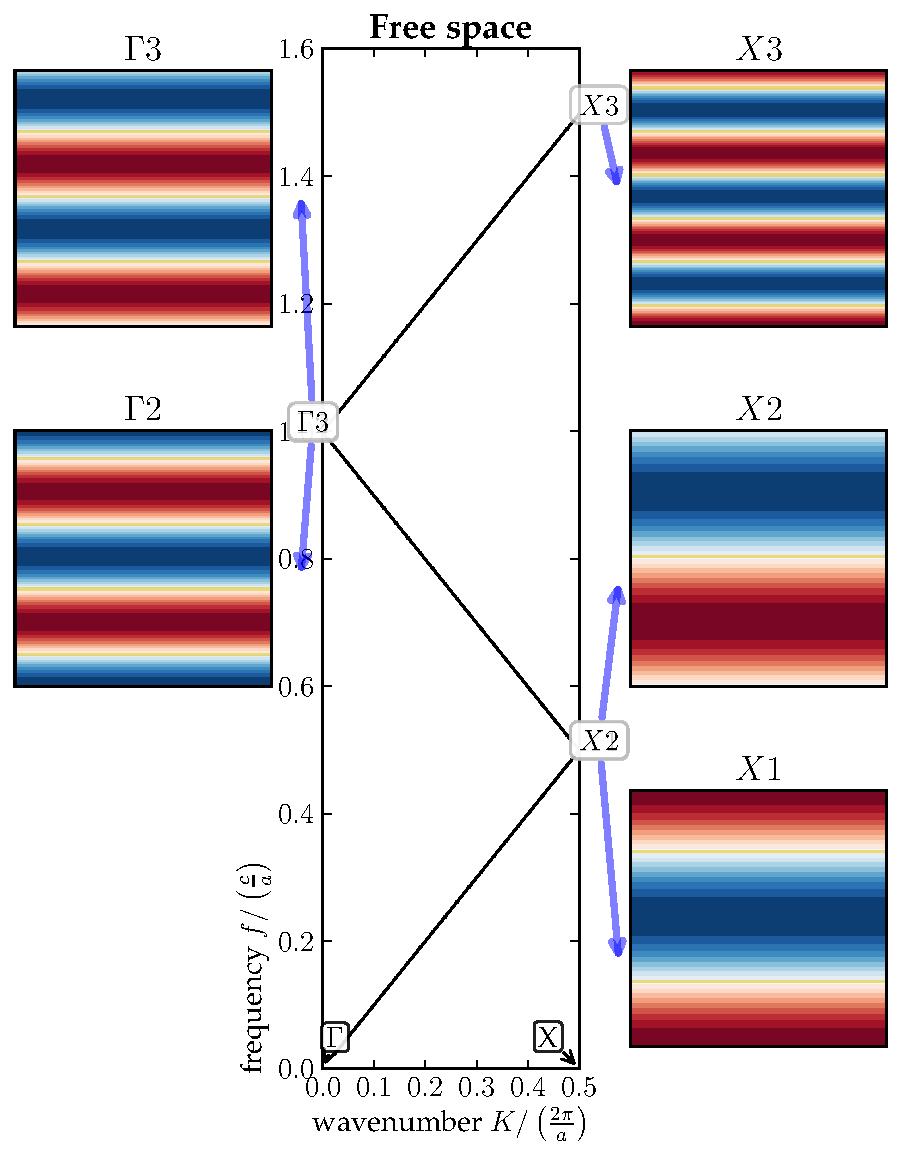
\includegraphics[width=10cm]{img/Slab_eps001_PWEM.pdf} \end{figure} \clearpage%{{{
\begin{figure} \caption{img/Slab\_eps012\_d15.pdf}  \centering 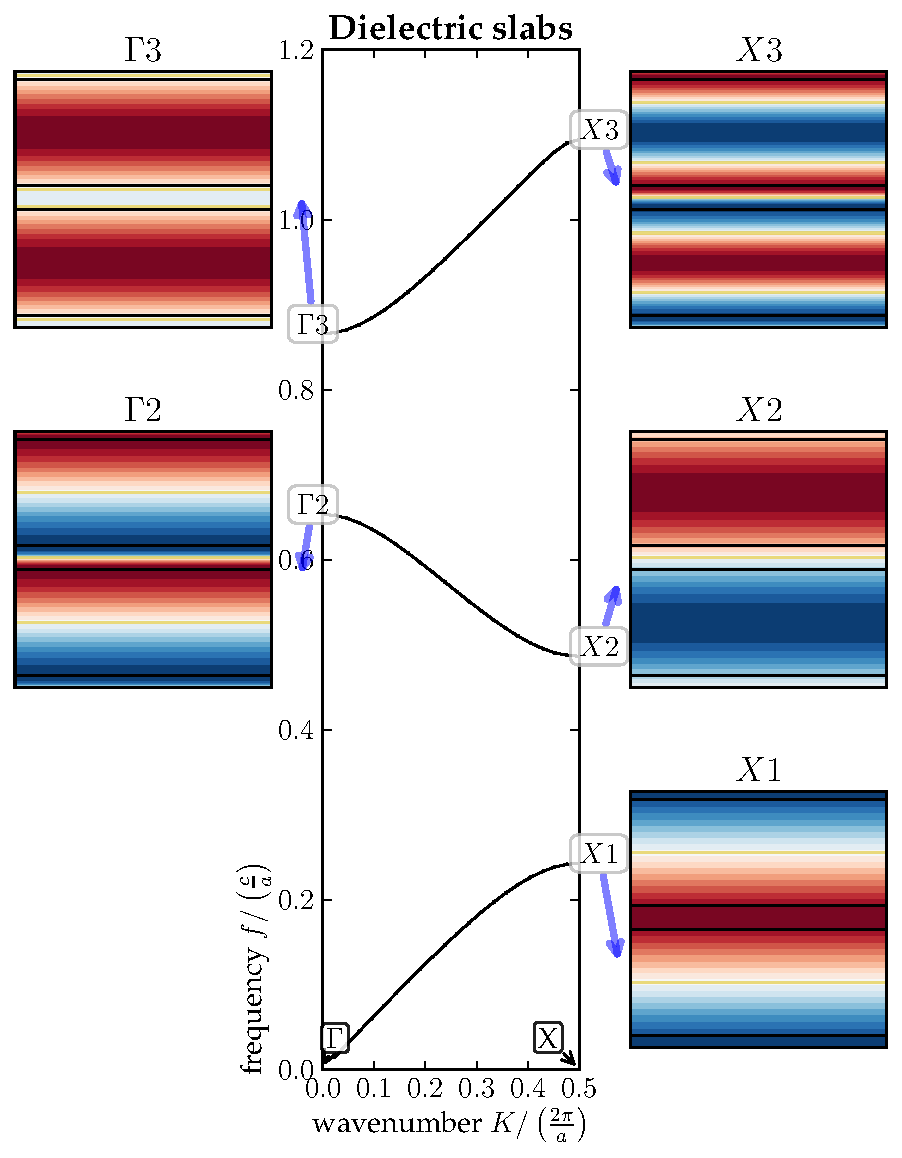
\includegraphics[width=10cm]{img/Slab_eps012_d15.pdf} \end{figure} \clearpage
\subsection{Finite planar structure with defect mode} % references to ->
A defect-mode transmission peak of 1.5\% energy transmission appears in the band gap.
It can be tuned from 173 to 184 GHz by application of electric field (40 kV/cm) to the defect STO layer \cite{skoromets2013}.
%}}}
\section{Wire medium} % references to ->
%{{{
\begin{figure} \caption{img/XCylWire\_a100r4.pdf}  \centering 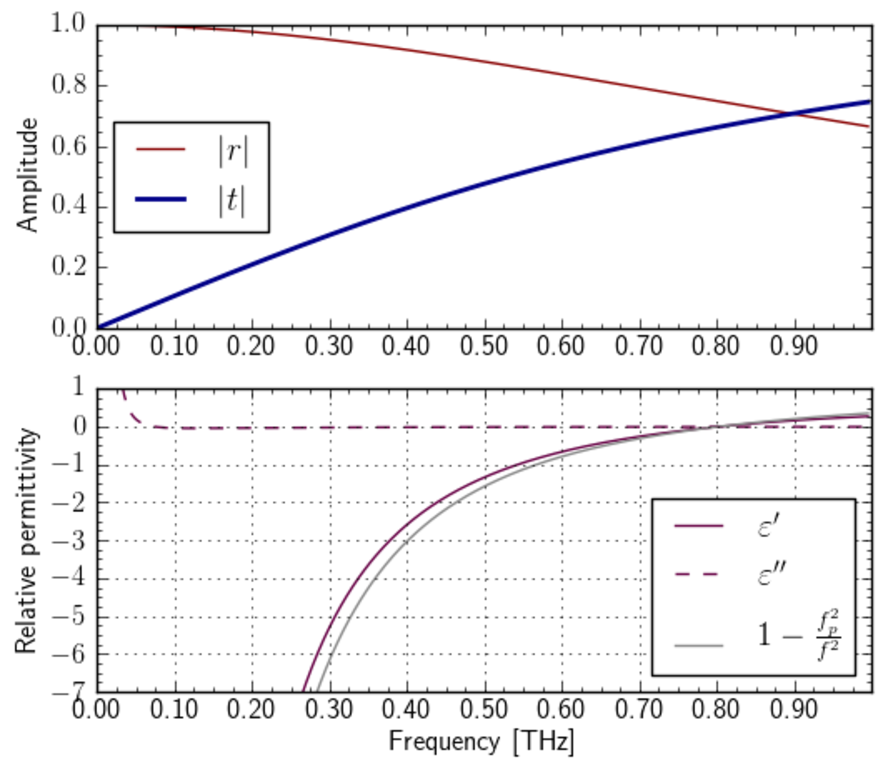
\includegraphics[width=10cm]{img/XCylWire_a100r4.pdf} \end{figure} \clearpage
\begin{figure} \caption{img/EWire\_plasmaF\_radiusscan.pdf}  \centering 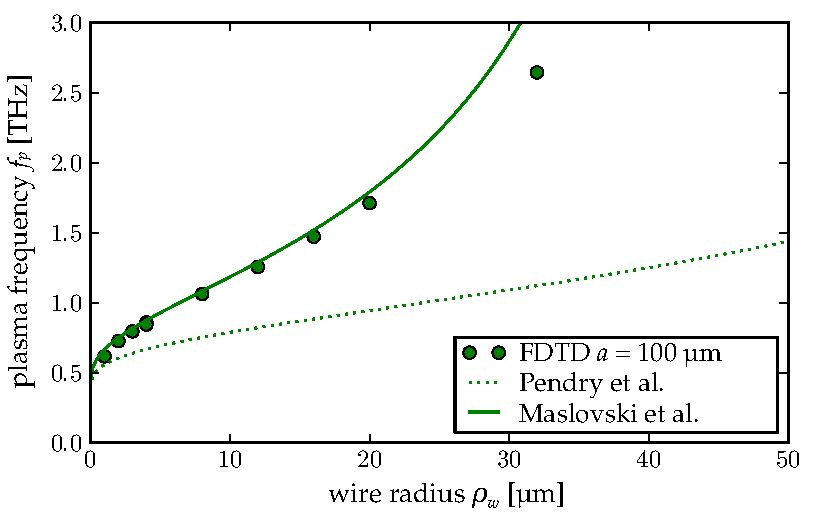
\includegraphics[width=10cm]{img/EWire_plasmaF_radiusscan.pdf} \end{figure} \clearpage
\begin{figure} \caption{img/EWire\_plasmaF\_spacingscan.pdf}  \centering 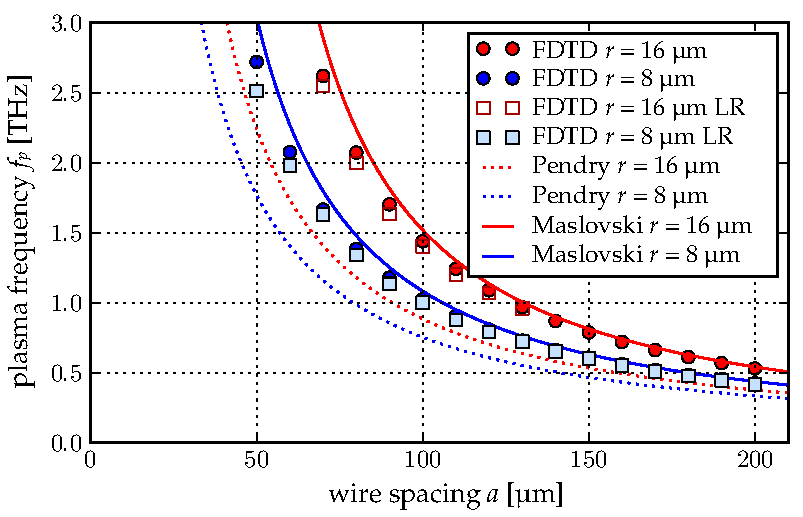
\includegraphics[width=10cm]{img/EWire_plasmaF_spacingscan.pdf} \end{figure} \clearpage
\begin{figure} \caption{img/EWire\_r03\_FDTDwide.pdf}  \centering 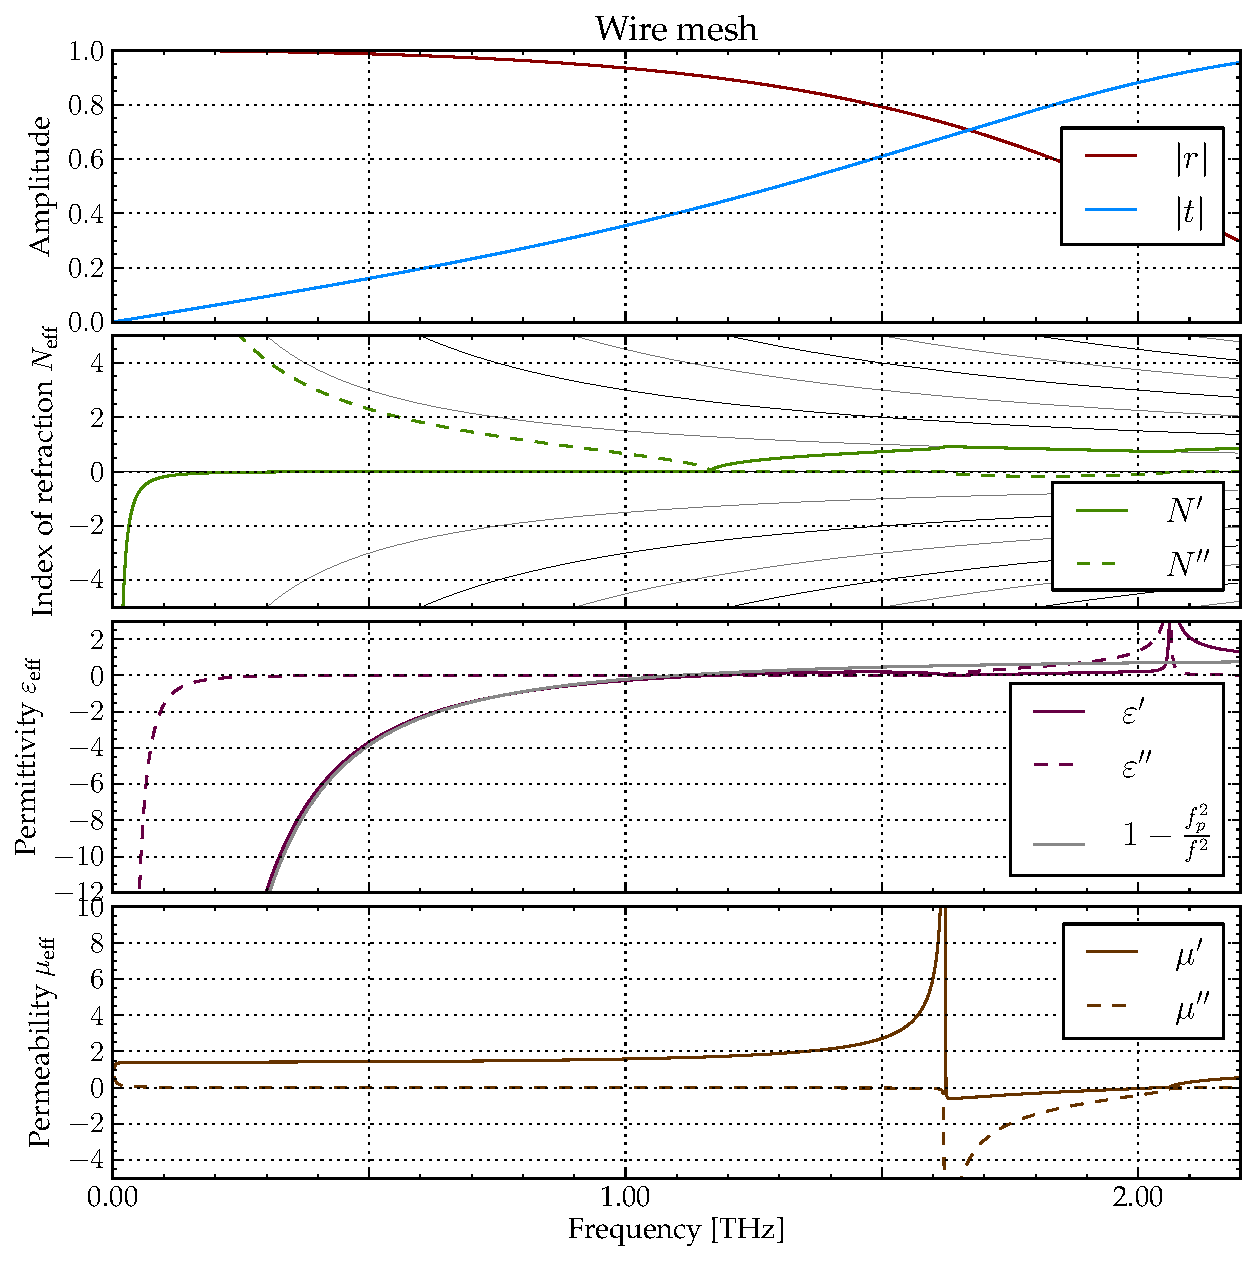
\includegraphics[width=10cm]{img/EWire_r03_FDTDwide.pdf} \end{figure} \clearpage
%}}}
\section{Metallic strips} % references to -> % note about plasmonic particles
\section{Metallic strip pair} % references to ->
\section{Split-ring resonator} % references to ->
\section{Dielectric sphere} % references to ->
%{{{
\begin{figure} \caption{img/Sphere\_eps100\_R25\_FDTD.pdf}  \centering 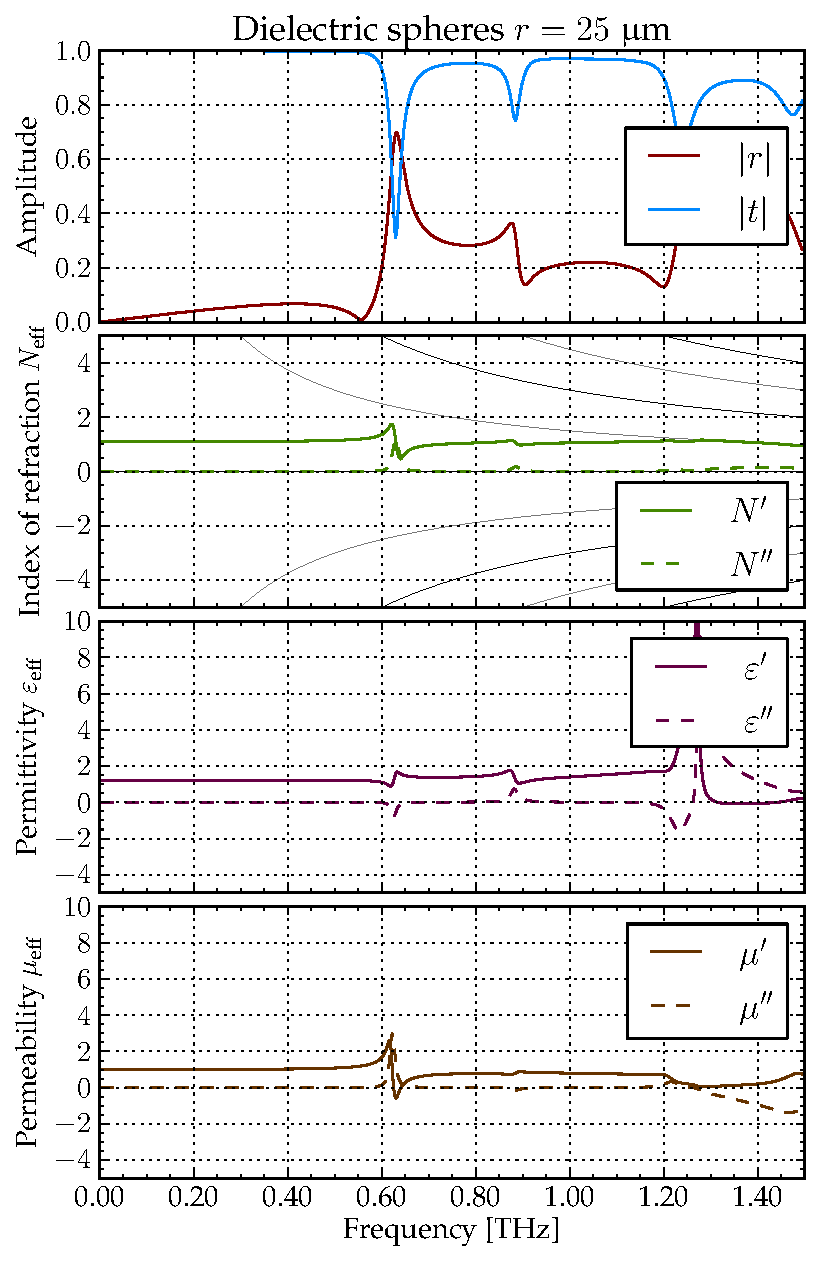
\includegraphics[width=10cm]{img/Sphere_eps100_R25_FDTD.pdf} \end{figure} \clearpage
\begin{figure} \caption{img/sphere\_Mie\_mode\_electric.pdf}  \centering 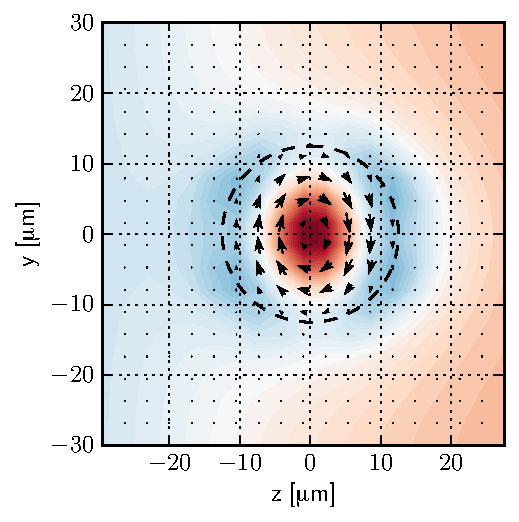
\includegraphics[width=10cm]{img/sphere_Mie_mode_electric.pdf} \end{figure} \clearpage
\begin{figure} \caption{img/sphere\_Mie\_mode\_magnetic.pdf}  \centering 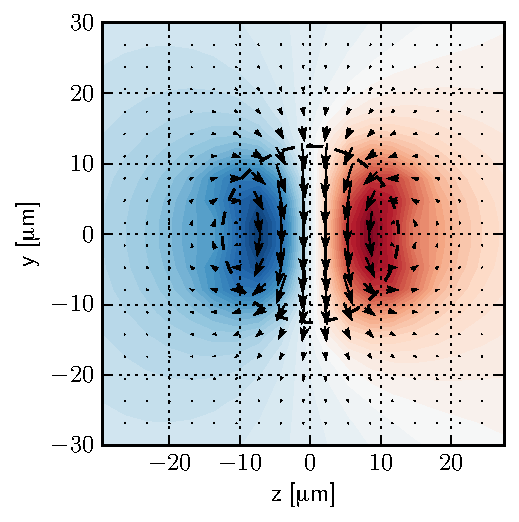
\includegraphics[width=10cm]{img/sphere_Mie_mode_magnetic.pdf} \end{figure} \clearpage
\begin{figure} \caption{img/Spheres\_FDTD\_experimentalConv.pdf}  \centering 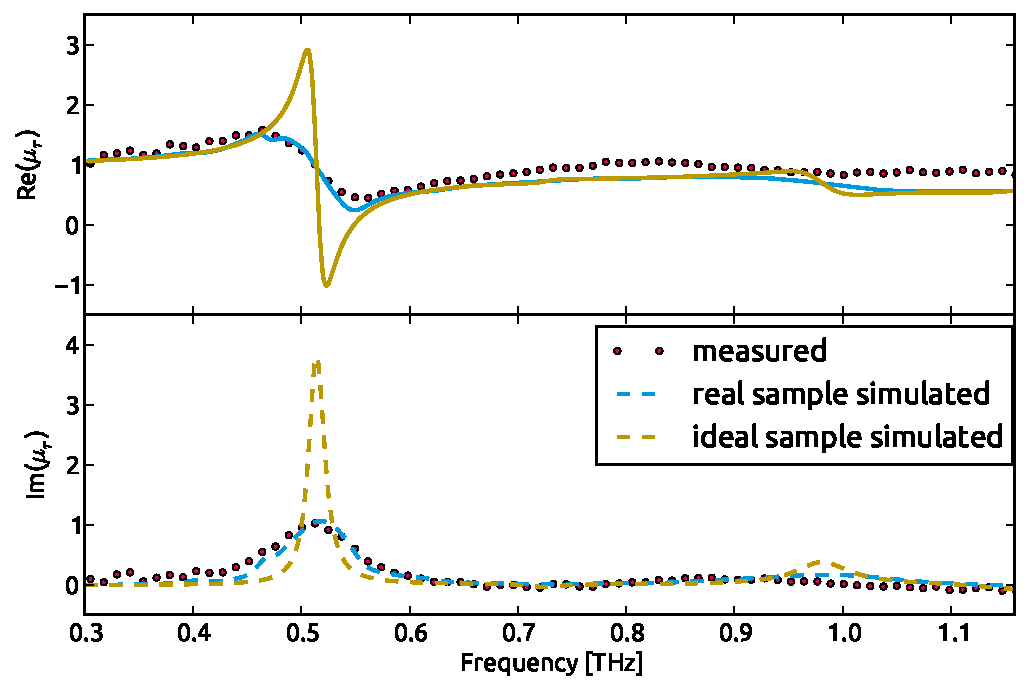
\includegraphics[width=10cm]{img/Spheres_FDTD_experimentalConv.pdf} \end{figure} \clearpage
%}}}
\section{SRRs and spheres in wire grid} % references to ->
%{{{
\begin{figure} \caption{img/SphereWire\_eps100\_R25\_FDTD.pdf}  \centering  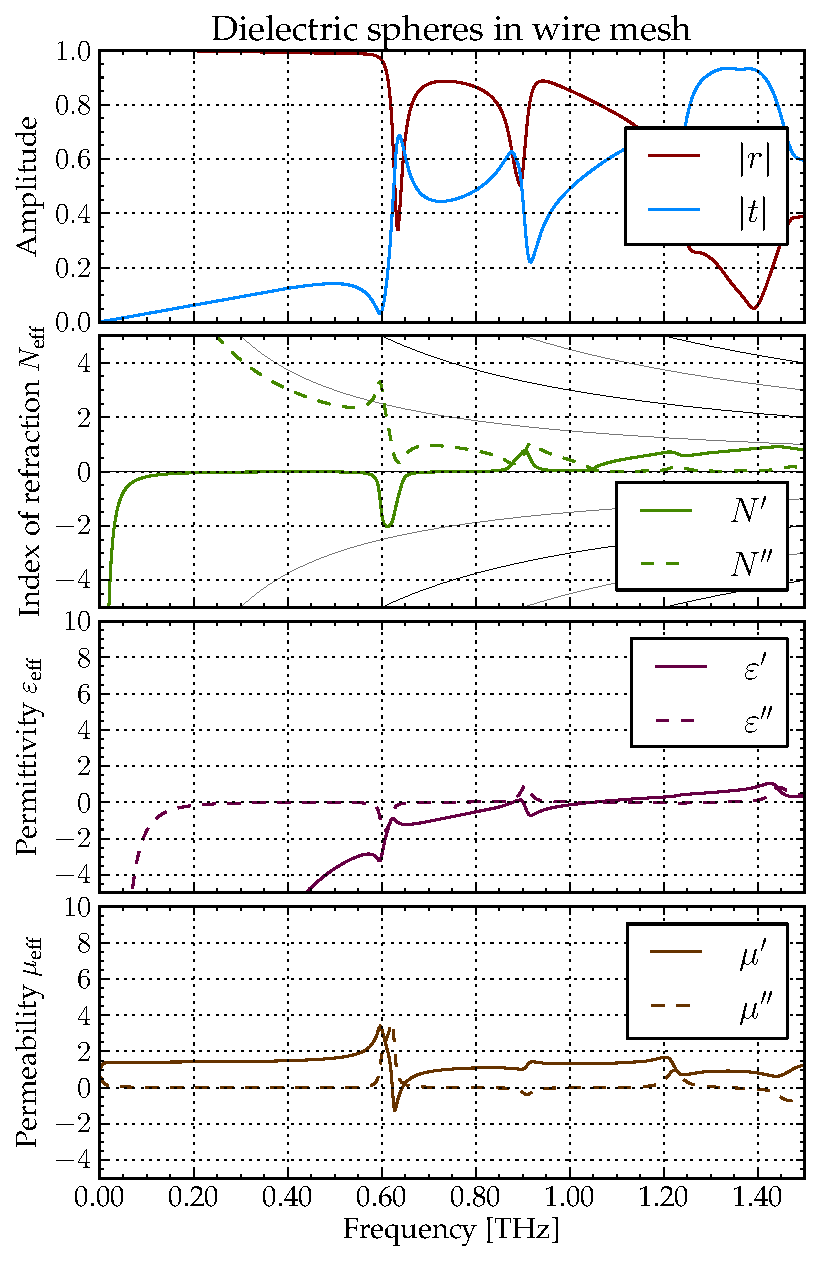
\includegraphics[width=10cm]{img/SphereWire_eps100_R25_FDTD.pdf} \end{figure} \clearpage
%}}}
\section{Dielectric rods parallel to magnetic field} % references to ->
%{{{
\begin{figure} \caption{img/HRods\_eps012\_R12\_PWEM.pdf}  \centering 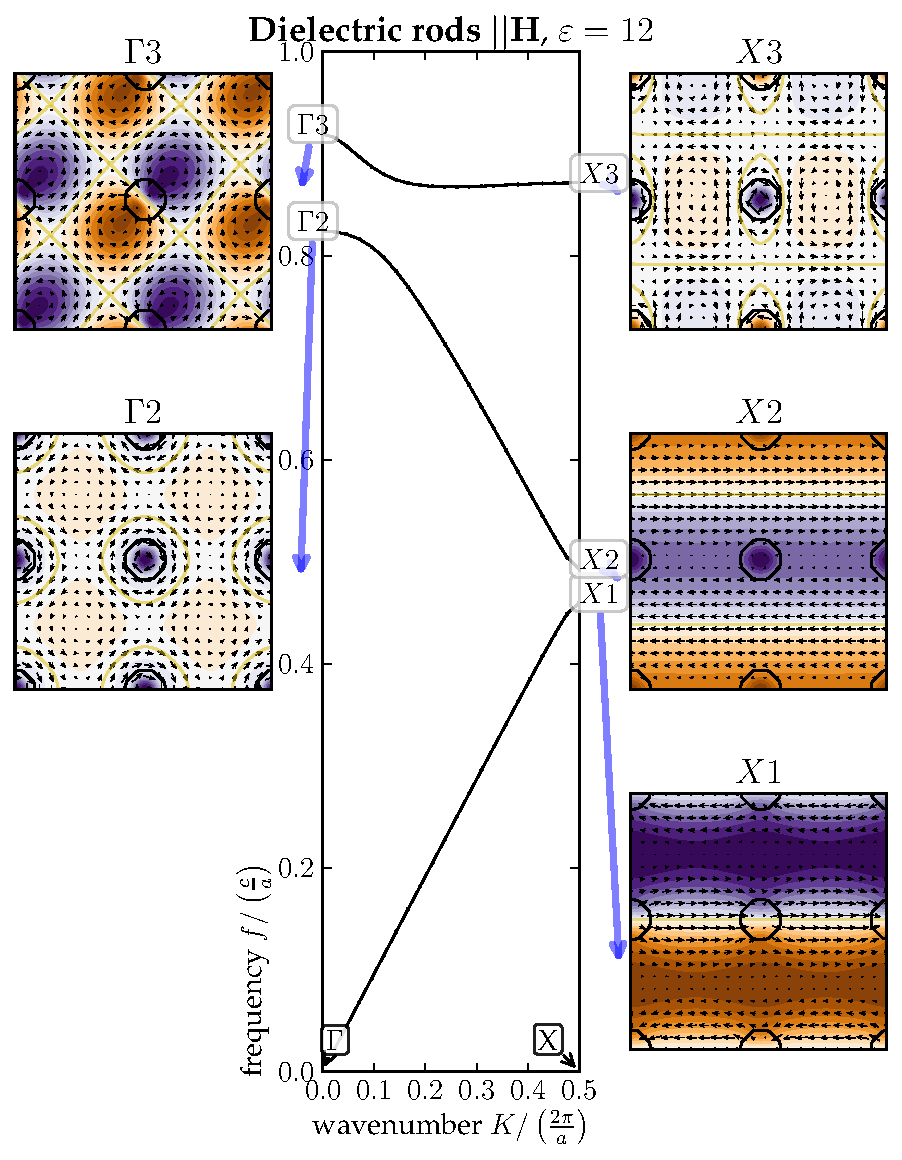
\includegraphics[width=10cm]{img/HRods_eps012_R12_PWEM.pdf} \end{figure} \clearpage
\begin{figure} \caption{img/HRods\_eps100\_R12\_FDTD.pdf}  \centering 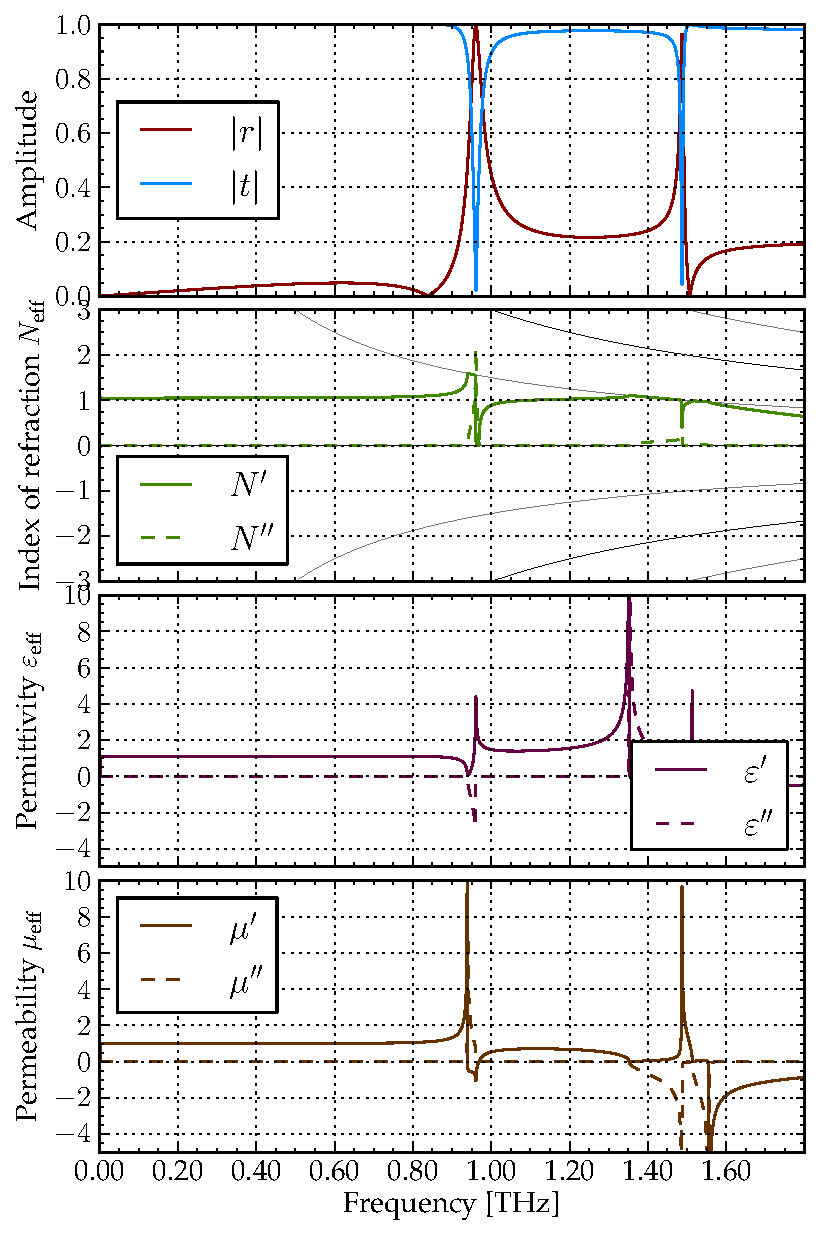
\includegraphics[width=10cm]{img/HRods_eps100_R12_FDTD.pdf} \end{figure} \clearpage
\begin{figure} \caption{img/HRods\_eps100\_R12\_PWEM.pdf}  \centering 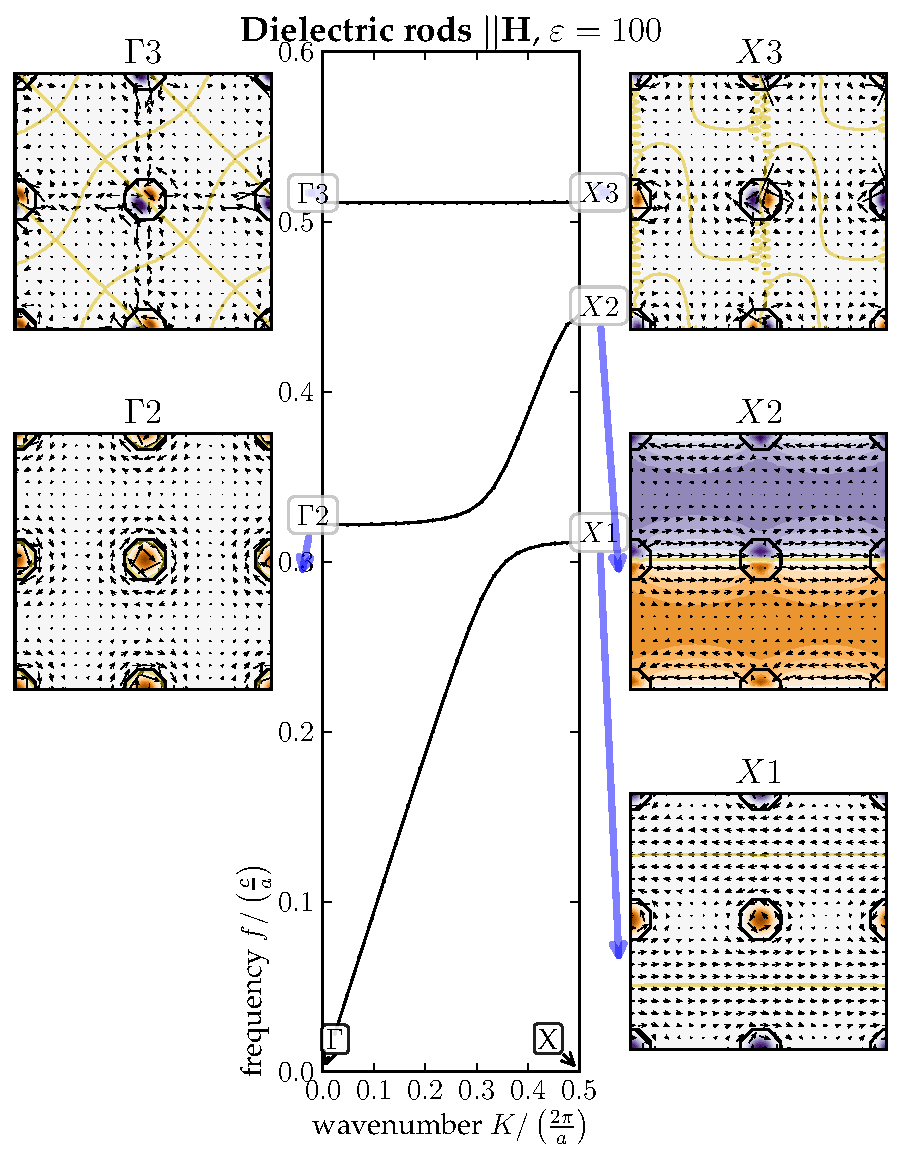
\includegraphics[width=10cm]{img/HRods_eps100_R12_PWEM.pdf} \end{figure} \clearpage
\begin{figure} \caption{img/HRods\_sketch.pdf}  \centering 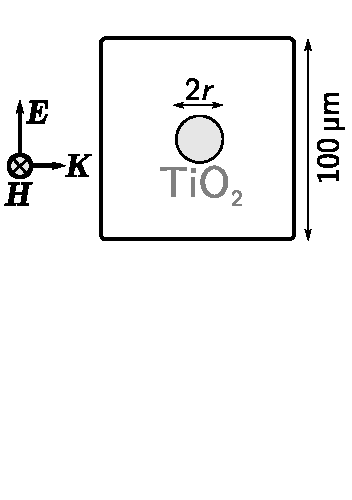
\includegraphics[width=10cm]{img/HRods_sketch.pdf} \end{figure} \clearpage
%}}}
\section{STO bar TODO} % references to ->
%{{{
\begin{figure} \caption{img/STOBarC\_modes3.pdf}  \centering 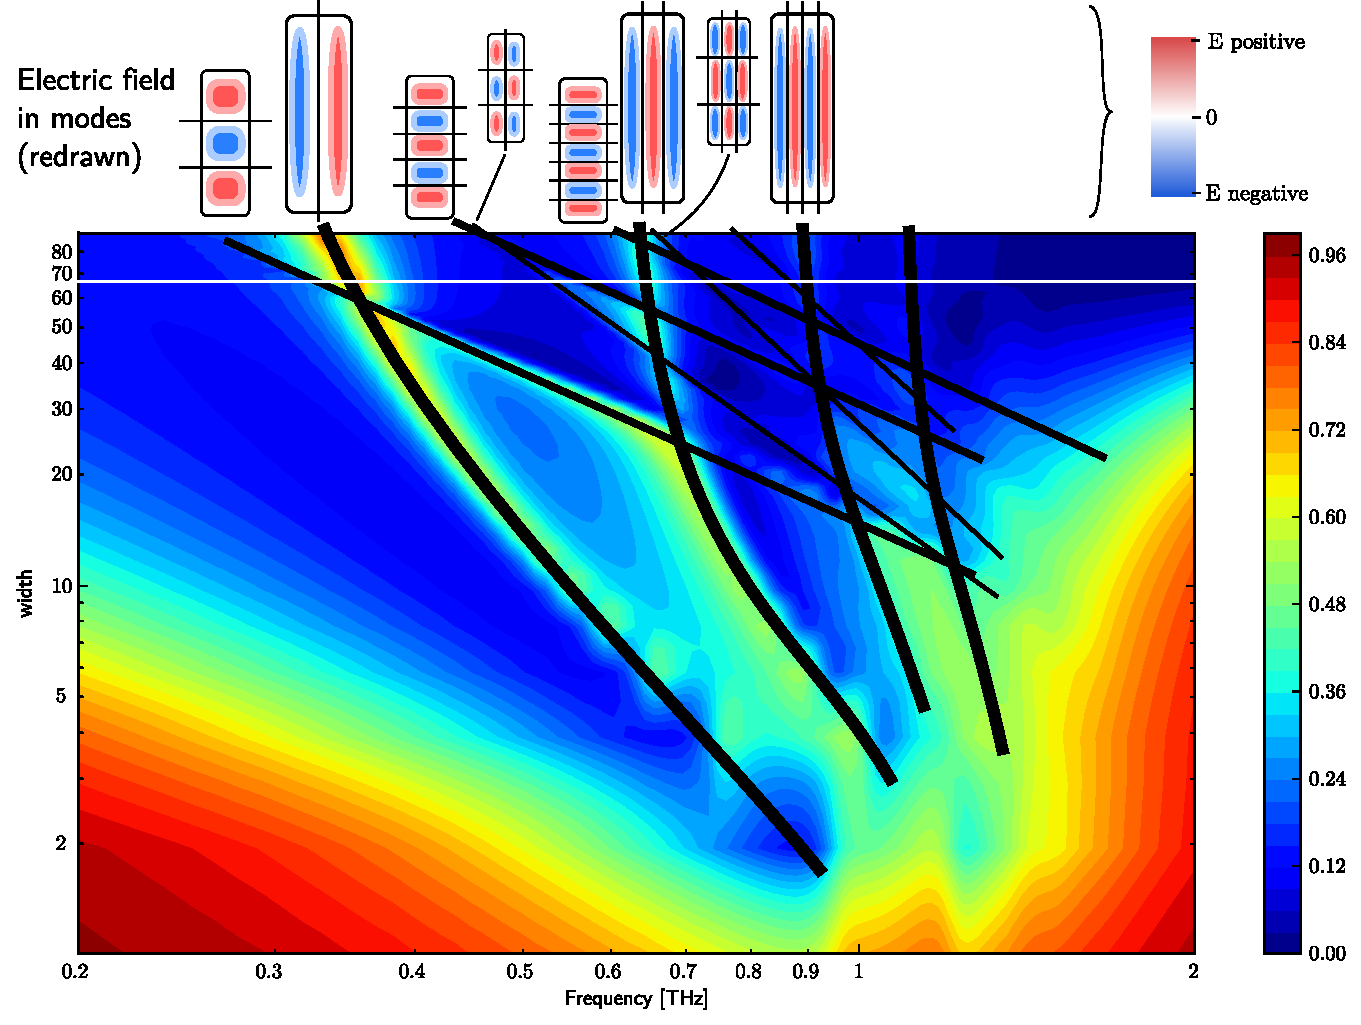
\includegraphics[width=10cm]{img/STOBarC_modes3.pdf} \end{figure} \clearpage
\begin{figure} \caption{img/STOBar\_photo\_narrow.pdf}  \centering 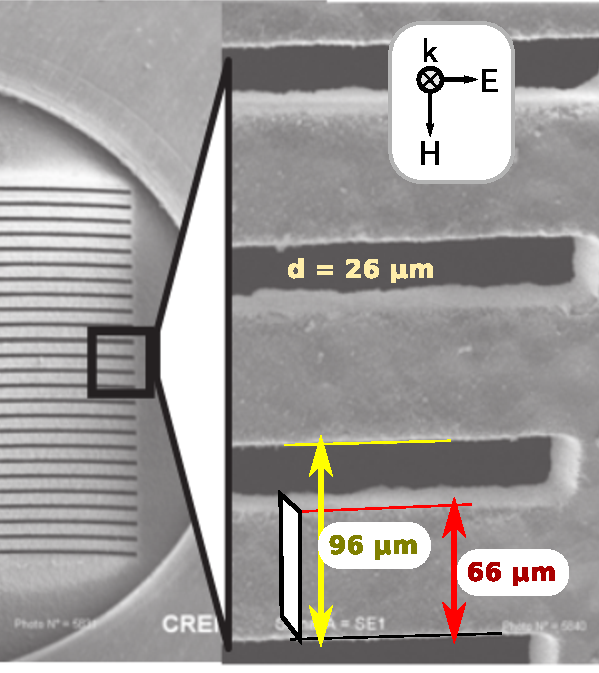
\includegraphics[width=10cm]{img/STOBar_photo_narrow.pdf} \end{figure} \clearpage
\begin{figure} \caption{img/STOBar\_photo.pdf}  \centering 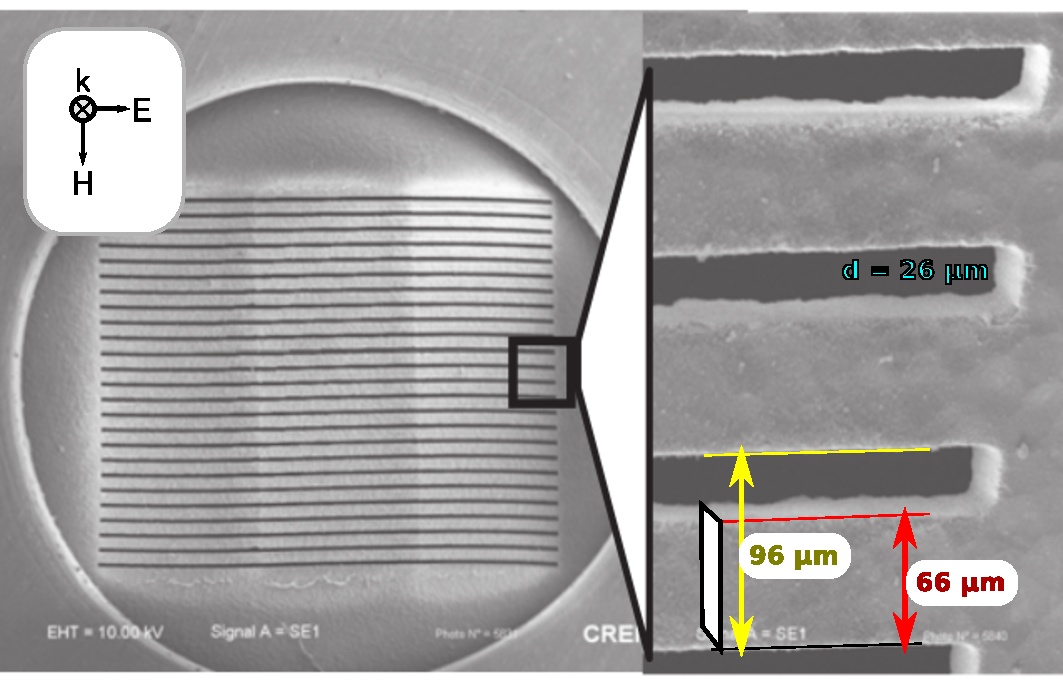
\includegraphics[width=10cm]{img/STOBar_photo.pdf} \end{figure} \clearpage
\begin{figure} \caption{img/STObar\_rt.pdf}  \centering 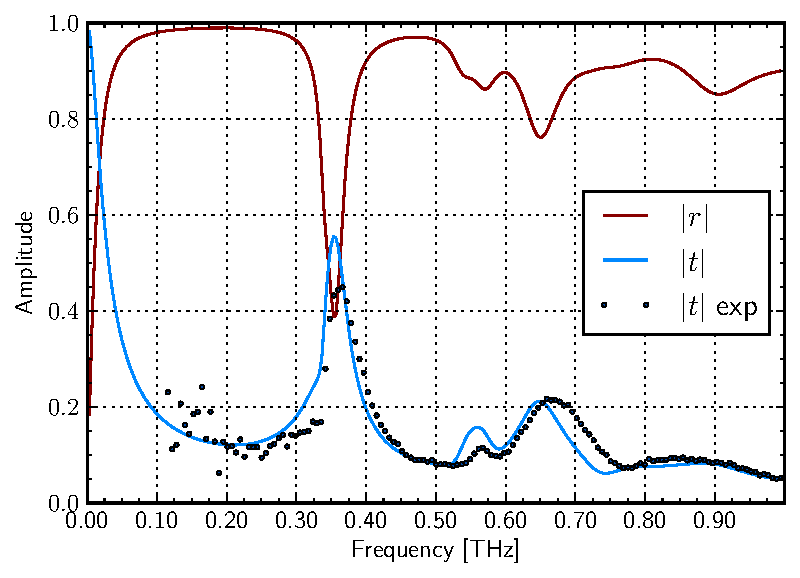
\includegraphics[width=10cm]{img/STObar_rt.pdf} \end{figure} \clearpage
%}}}
\section{Dielectric rods parallel to electric field} % references to ->
%{{{
% TODO refereence  also to \cite{valdivia2012} and \cite{shi2007}
\begin{figure} \caption{img/EBars\_STO\_sketch.pdf}  \centering 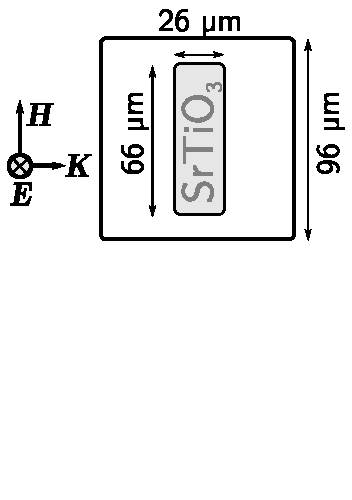
\includegraphics[width=10cm]{img/EBars_STO_sketch.pdf} \end{figure} \clearpage

\begin{figure} \caption{img/ERods\_1st\_and\_2nd\_Mie\_resonance.pdf}  \centering 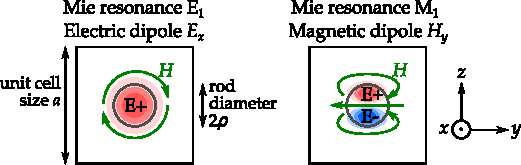
\includegraphics[width=10cm]{img/ERods_1st_and_2nd_Mie_resonance.pdf} \end{figure} \clearpage

\begin{figure} \caption{img/ERods\_eps100\_double\_a100a080\_FDTD.pdf}  \centering 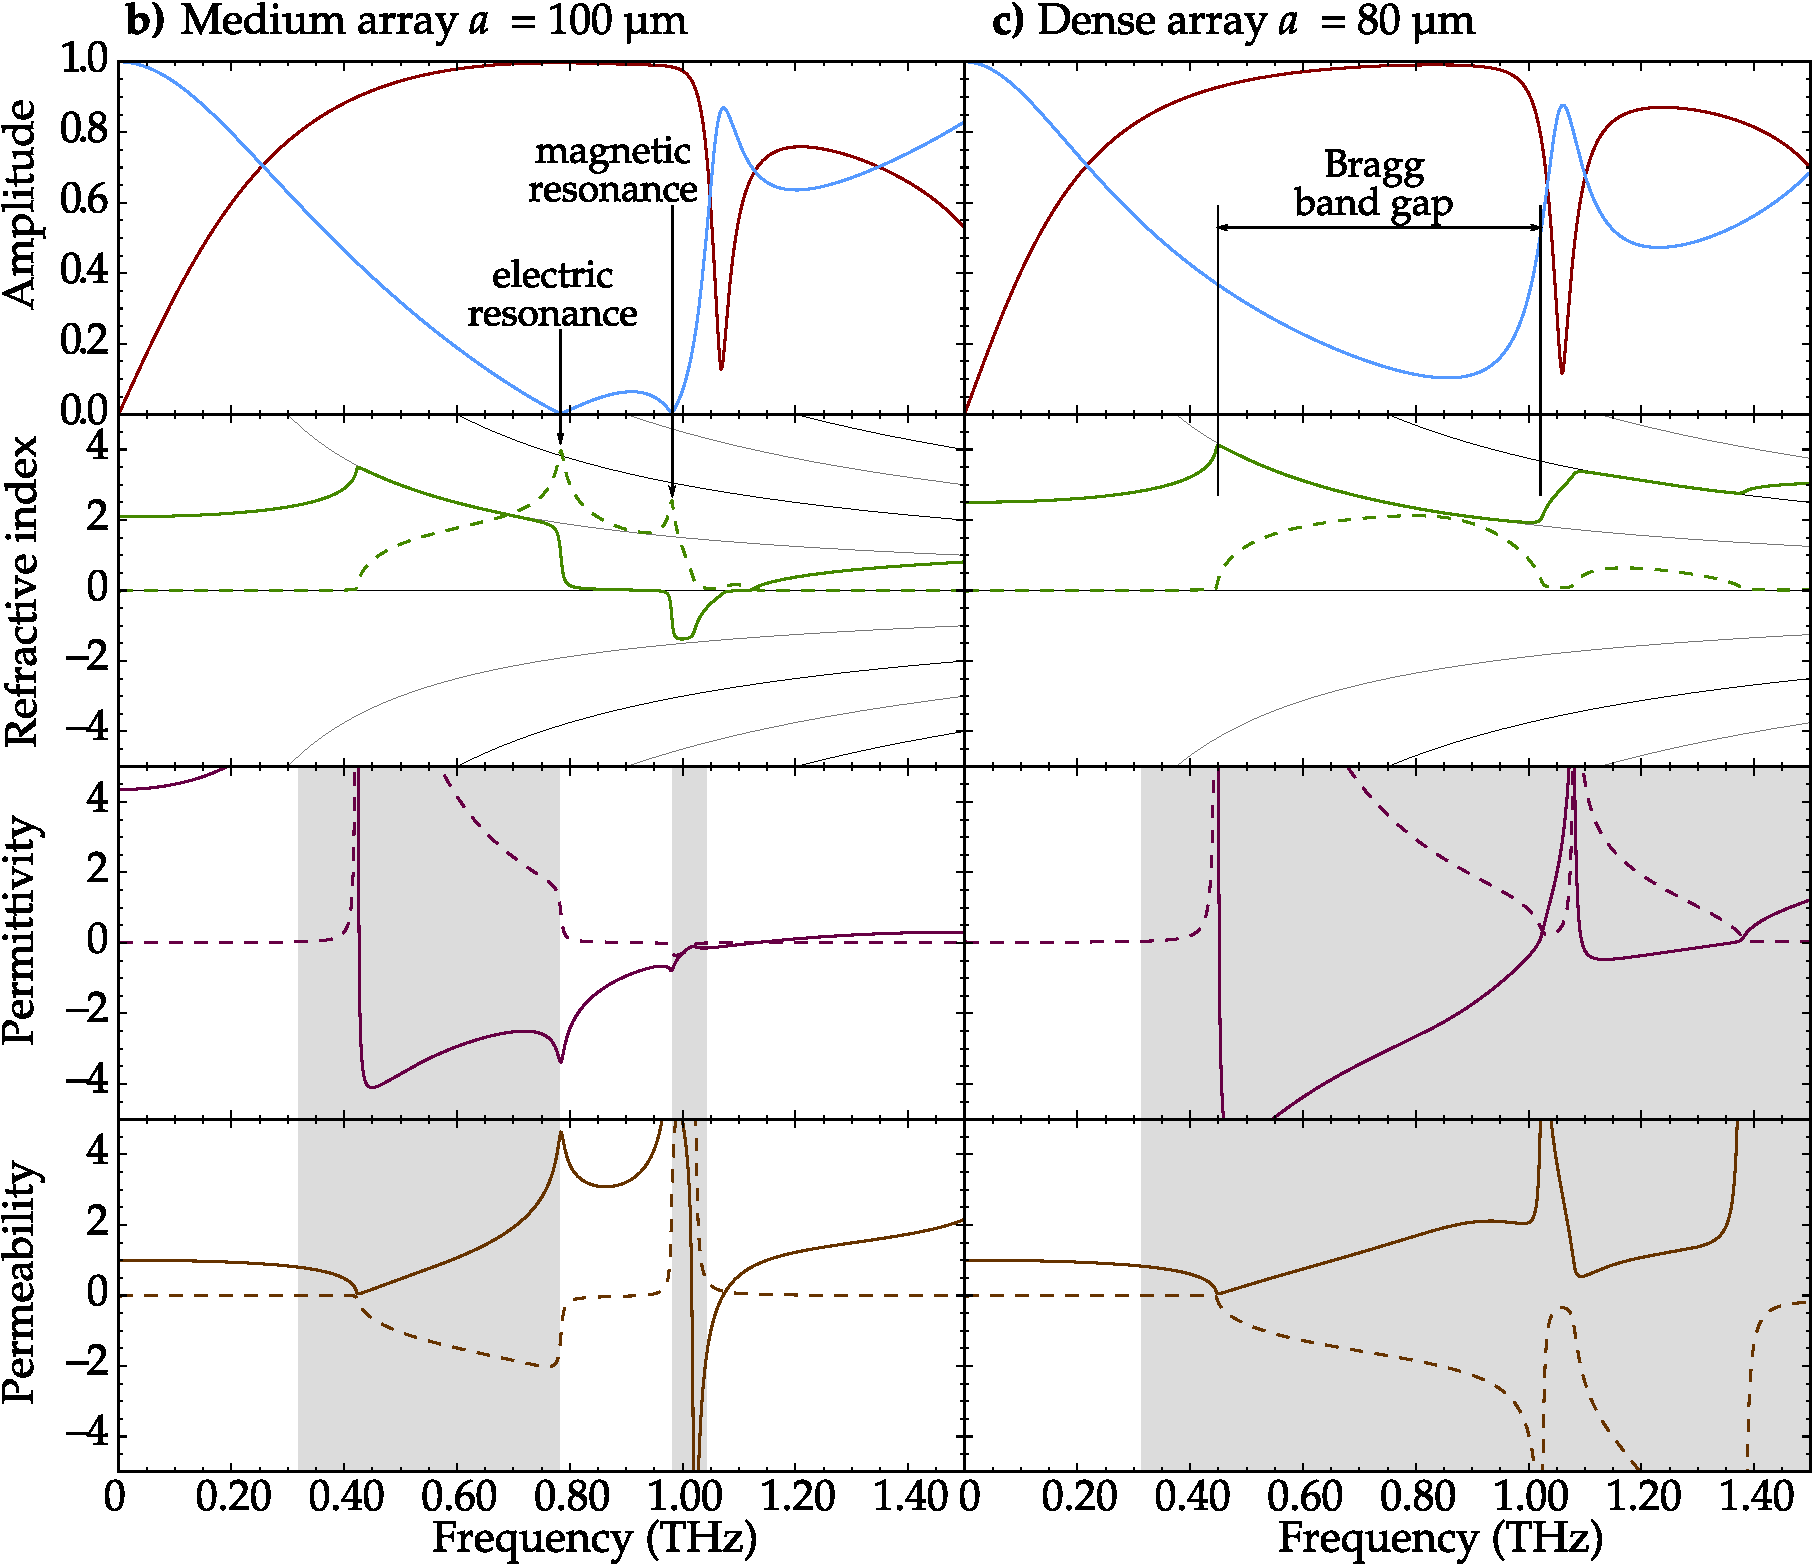
\includegraphics[width=10cm]{img/ERods_eps100_double_a100a080_FDTD.pdf} \end{figure} \clearpage

\begin{figure} \caption{img/sim\_ampli\_debug\_band.pdf}  \centering 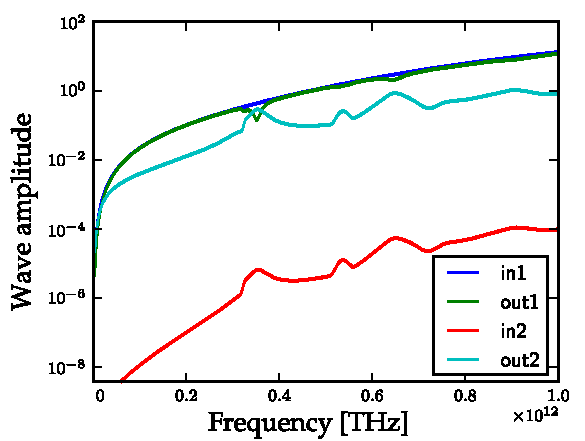
\includegraphics[width=10cm]{img/sim_ampli_debug_band.pdf} \end{figure} \clearpage
\begin{figure} \caption{img/sim\_screen.pdf}  \centering 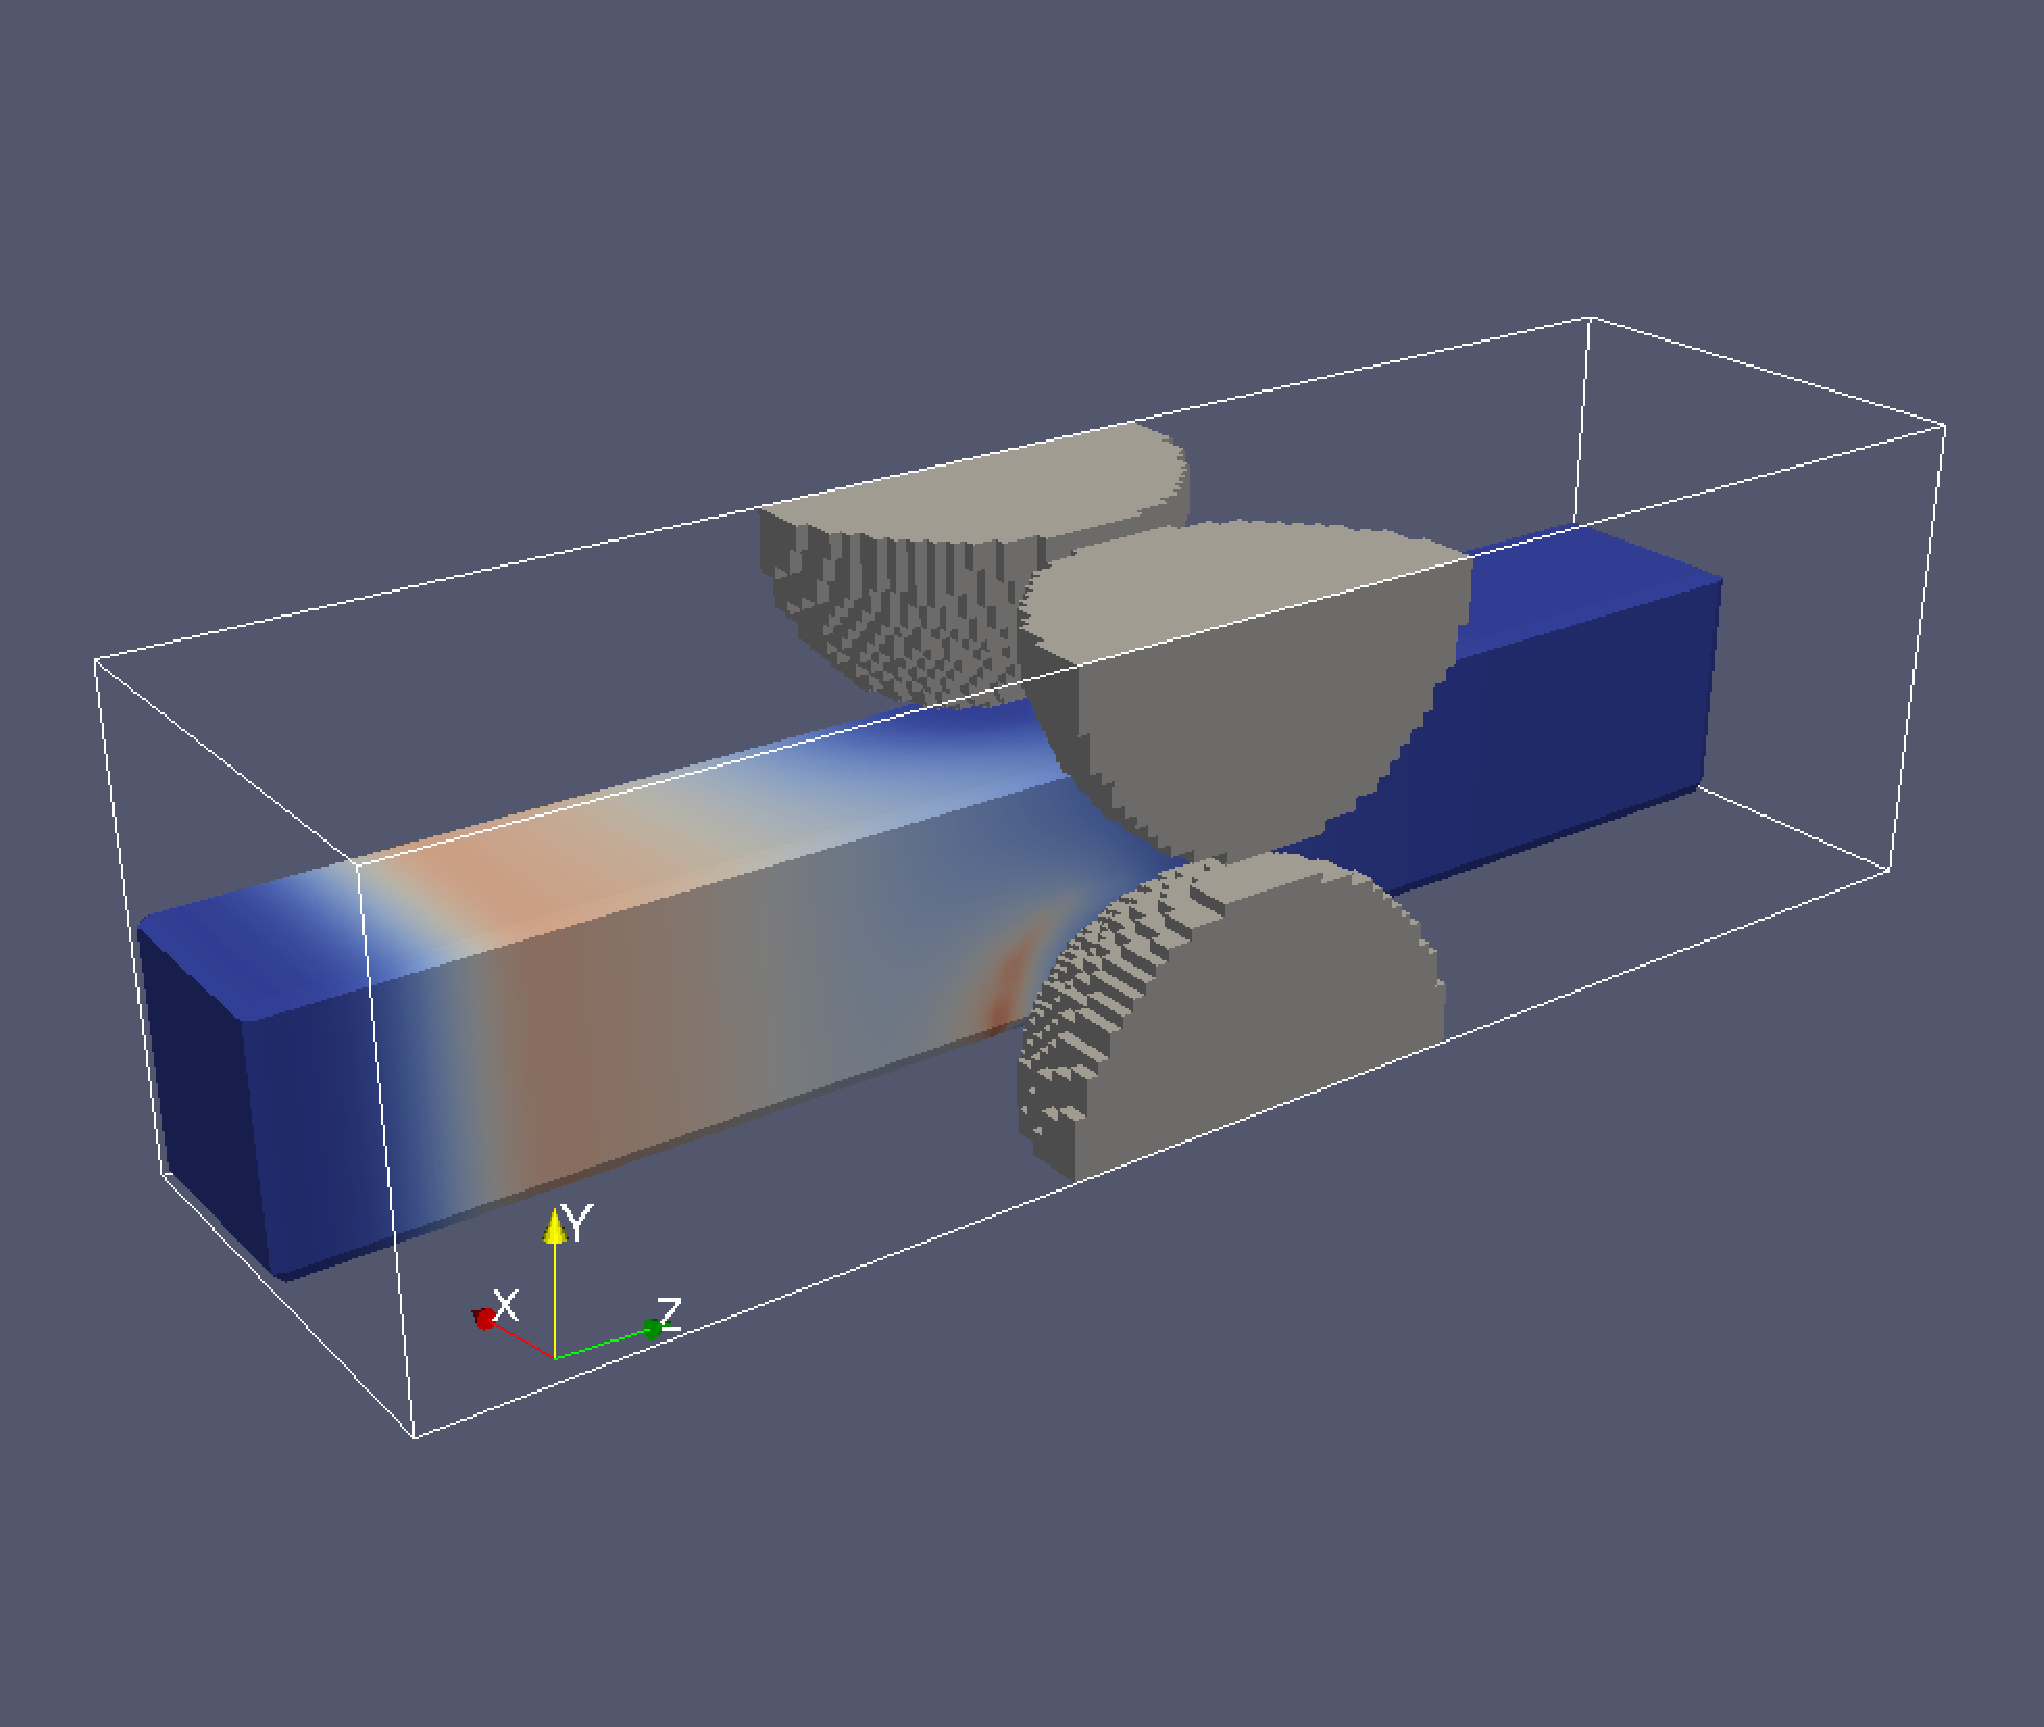
\includegraphics[width=10cm]{img/sim_screen.pdf} \end{figure} \clearpage
\begin{figure} \caption{img/sim\_separating\_wave.pdf}  \centering 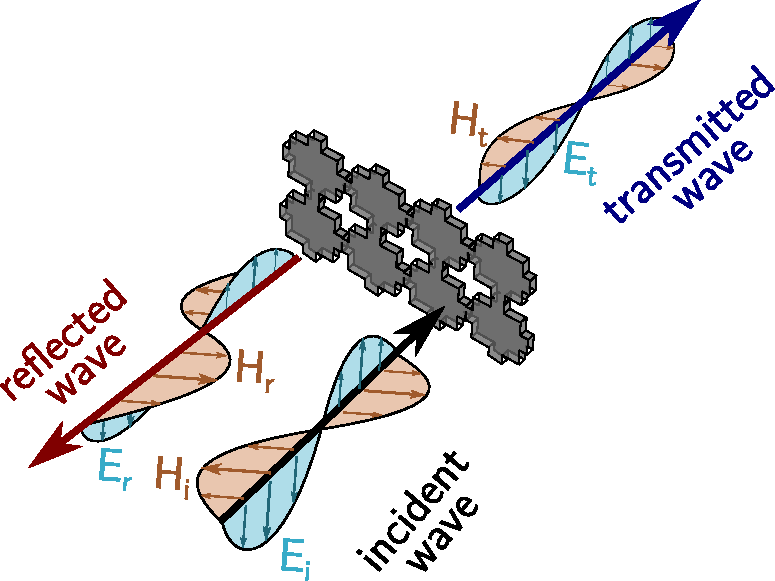
\includegraphics[width=10cm]{img/sim_separating_wave.pdf} \end{figure} \clearpage
\begin{figure} \caption{img/sim\_timedomain\_debug.pdf}  \centering 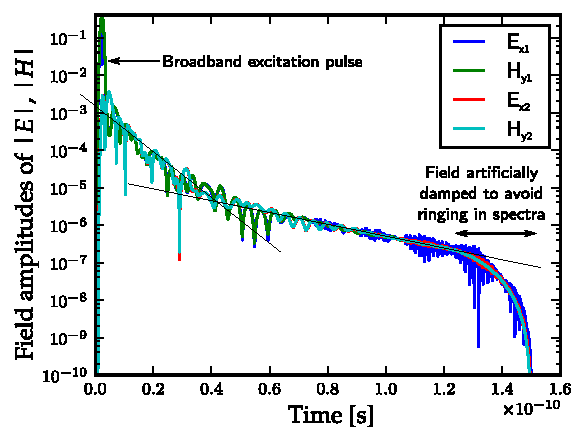
\includegraphics[width=10cm]{img/sim_timedomain_debug.pdf} \end{figure} \clearpage

\begin{figure} \caption{img/ERods\_sketch\_of\_separate\_spectra\_to\_continuous\_scan.pdf}  \centering 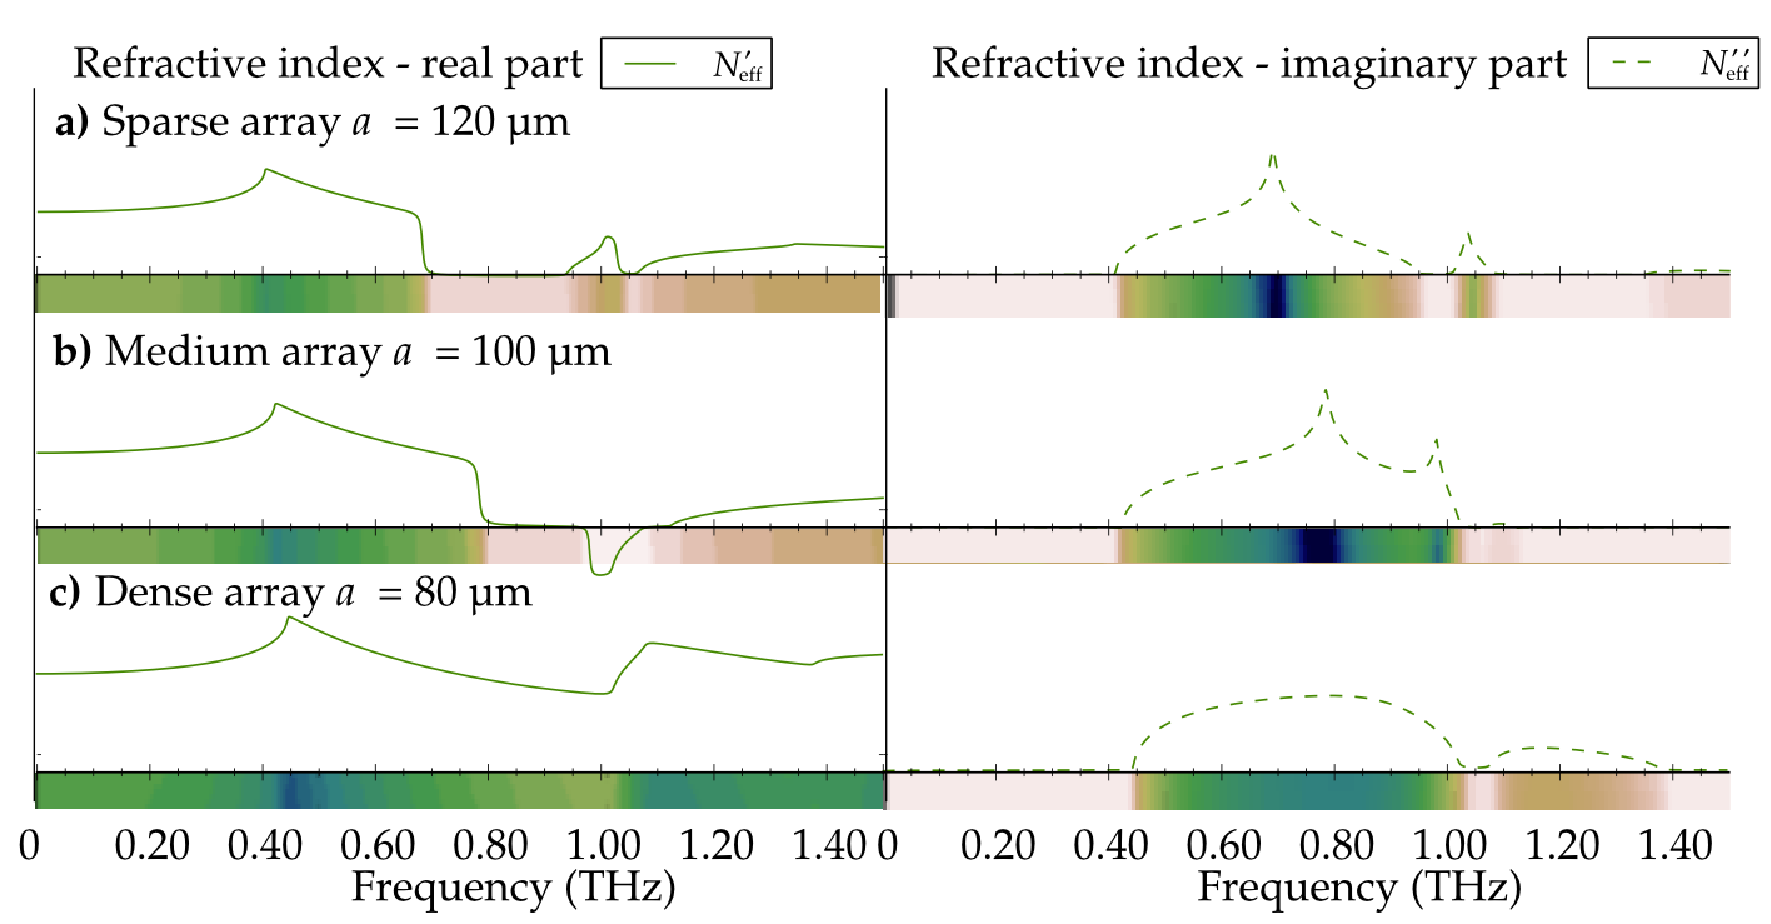
\includegraphics[width=10cm]{img/ERods_sketch_of_separate_spectra_to_continuous_scan.pdf} \end{figure} \clearpage
\begin{figure} \caption{img/ERods\_eps100\_spacingscan\_Nim.pdf}  \centering 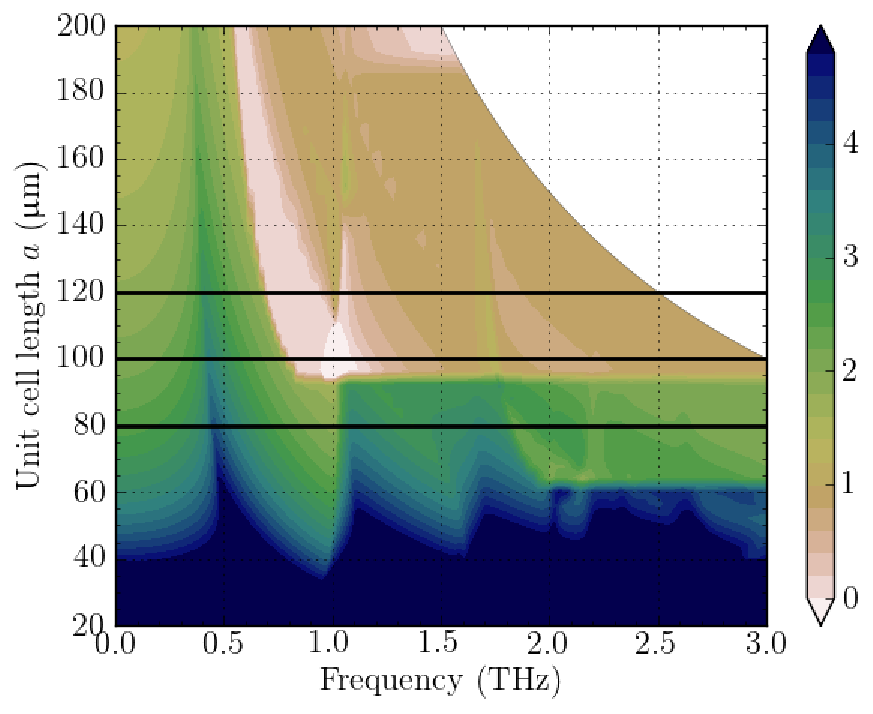
\includegraphics[width=10cm]{img/ERods_eps100_spacingscan_Nim.pdf} \end{figure} \clearpage
\begin{figure} \caption{img/ERods\_eps100\_spacingscan\_Nre.pdf}  \centering 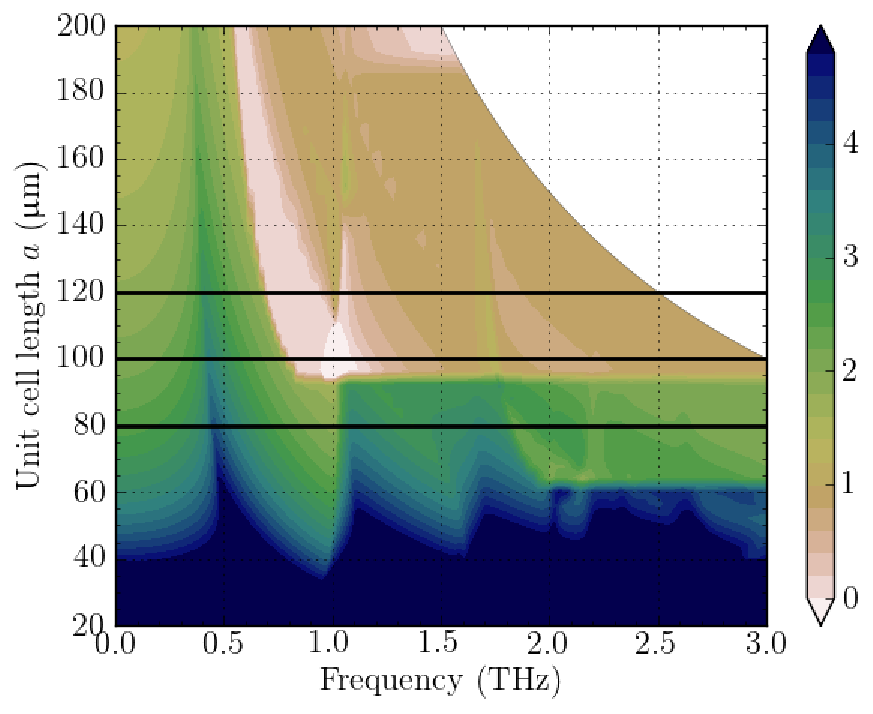
\includegraphics[width=10cm]{img/ERods_eps100_spacingscan_Nre.pdf} \end{figure} \clearpage
\begin{figure} \caption{img/ERods\_eps100\_spacingscan\_drawn\_bands.pdf}  \centering 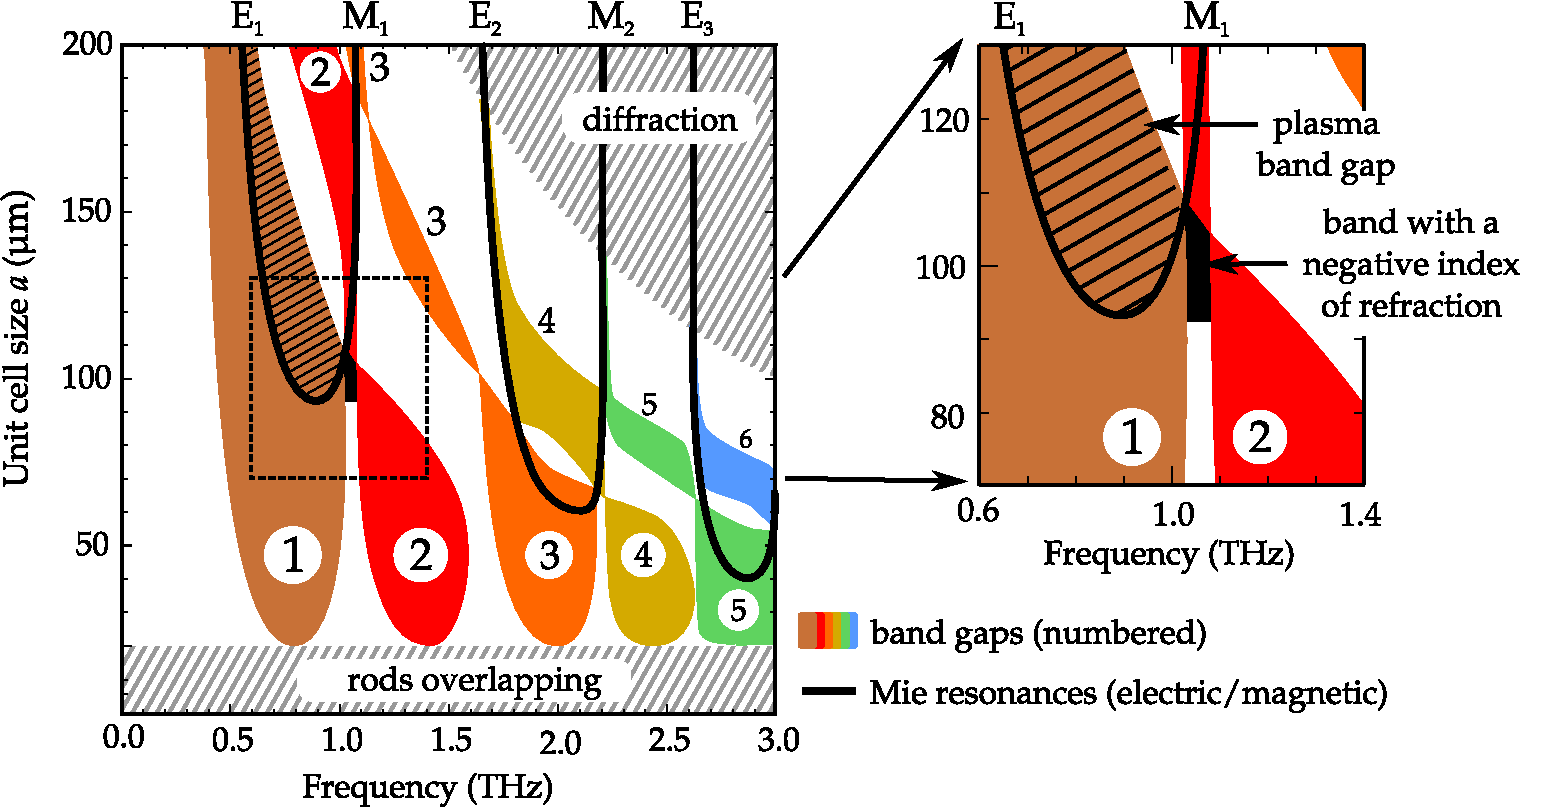
\includegraphics[width=10cm]{img/ERods_eps100_spacingscan_drawn_bands.pdf} \end{figure} \clearpage
\begin{figure} \caption{img/ERods\_eps030\_spacingscan\_drawn\_bands.pdf} \centering 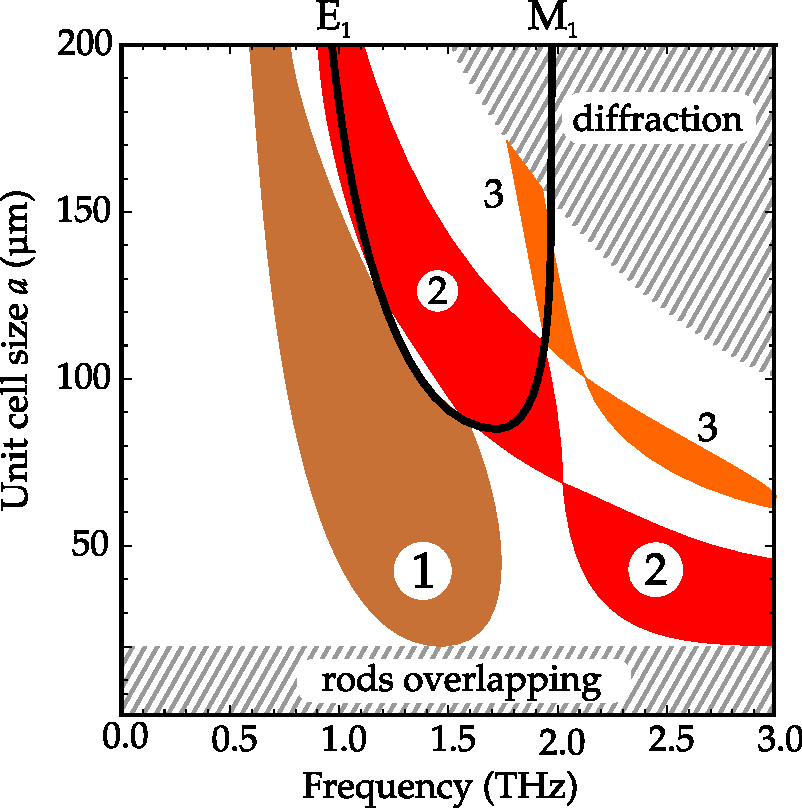
\includegraphics[width=10cm]{img/ERods_eps030_spacingscan_drawn_bands.pdf} \end{figure} \clearpage

\begin{figure} \caption{img/ERods\_eps100\_R11\_PWEM.pdf}  \centering 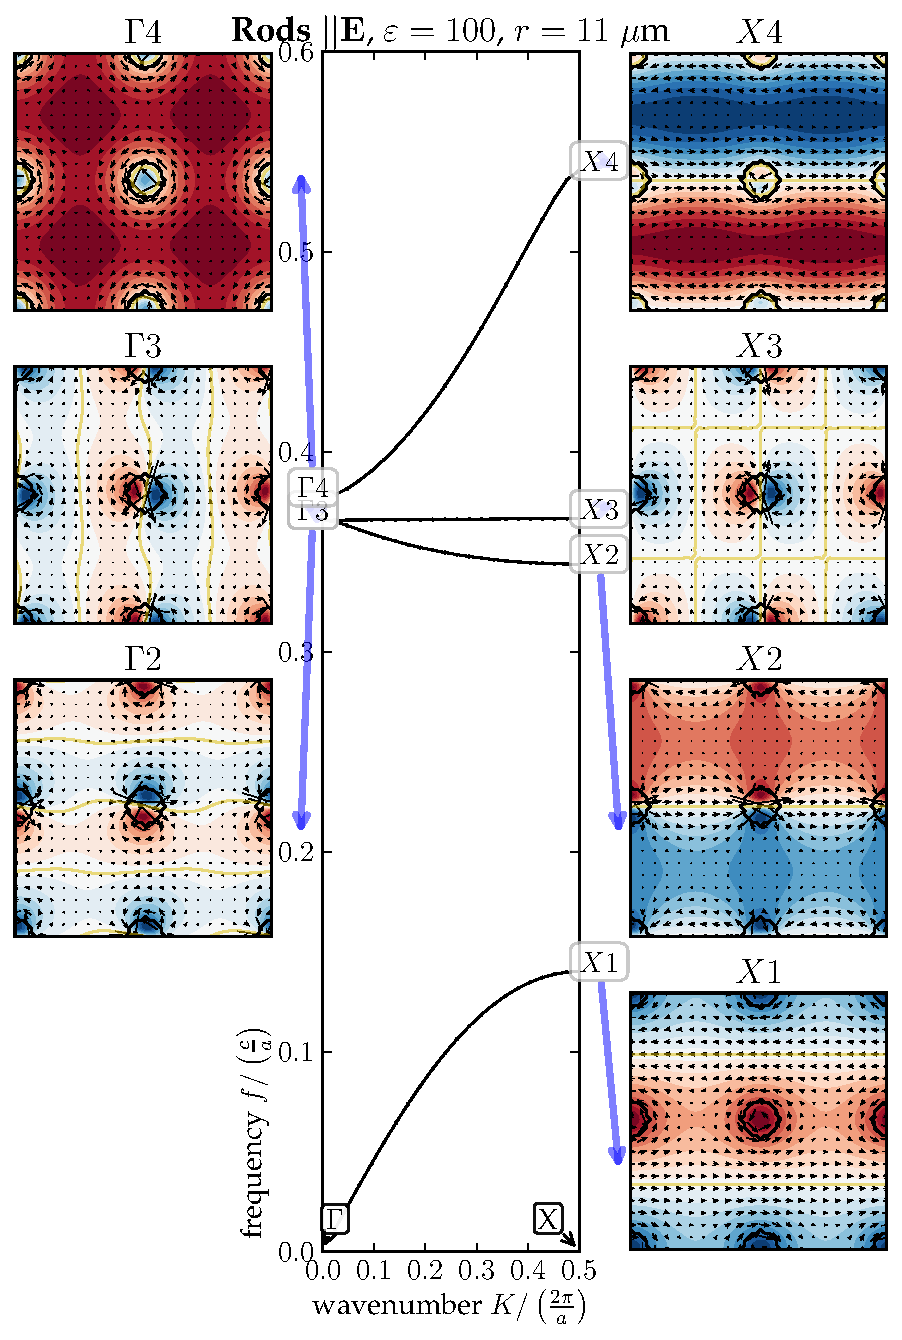
\includegraphics[width=10cm]{img/ERods_eps100_R11_PWEM.pdf} \end{figure} \clearpage
\begin{figure} \caption{img/ERods\_eps100\_single\_a120\_FDTD.pdf}  \centering 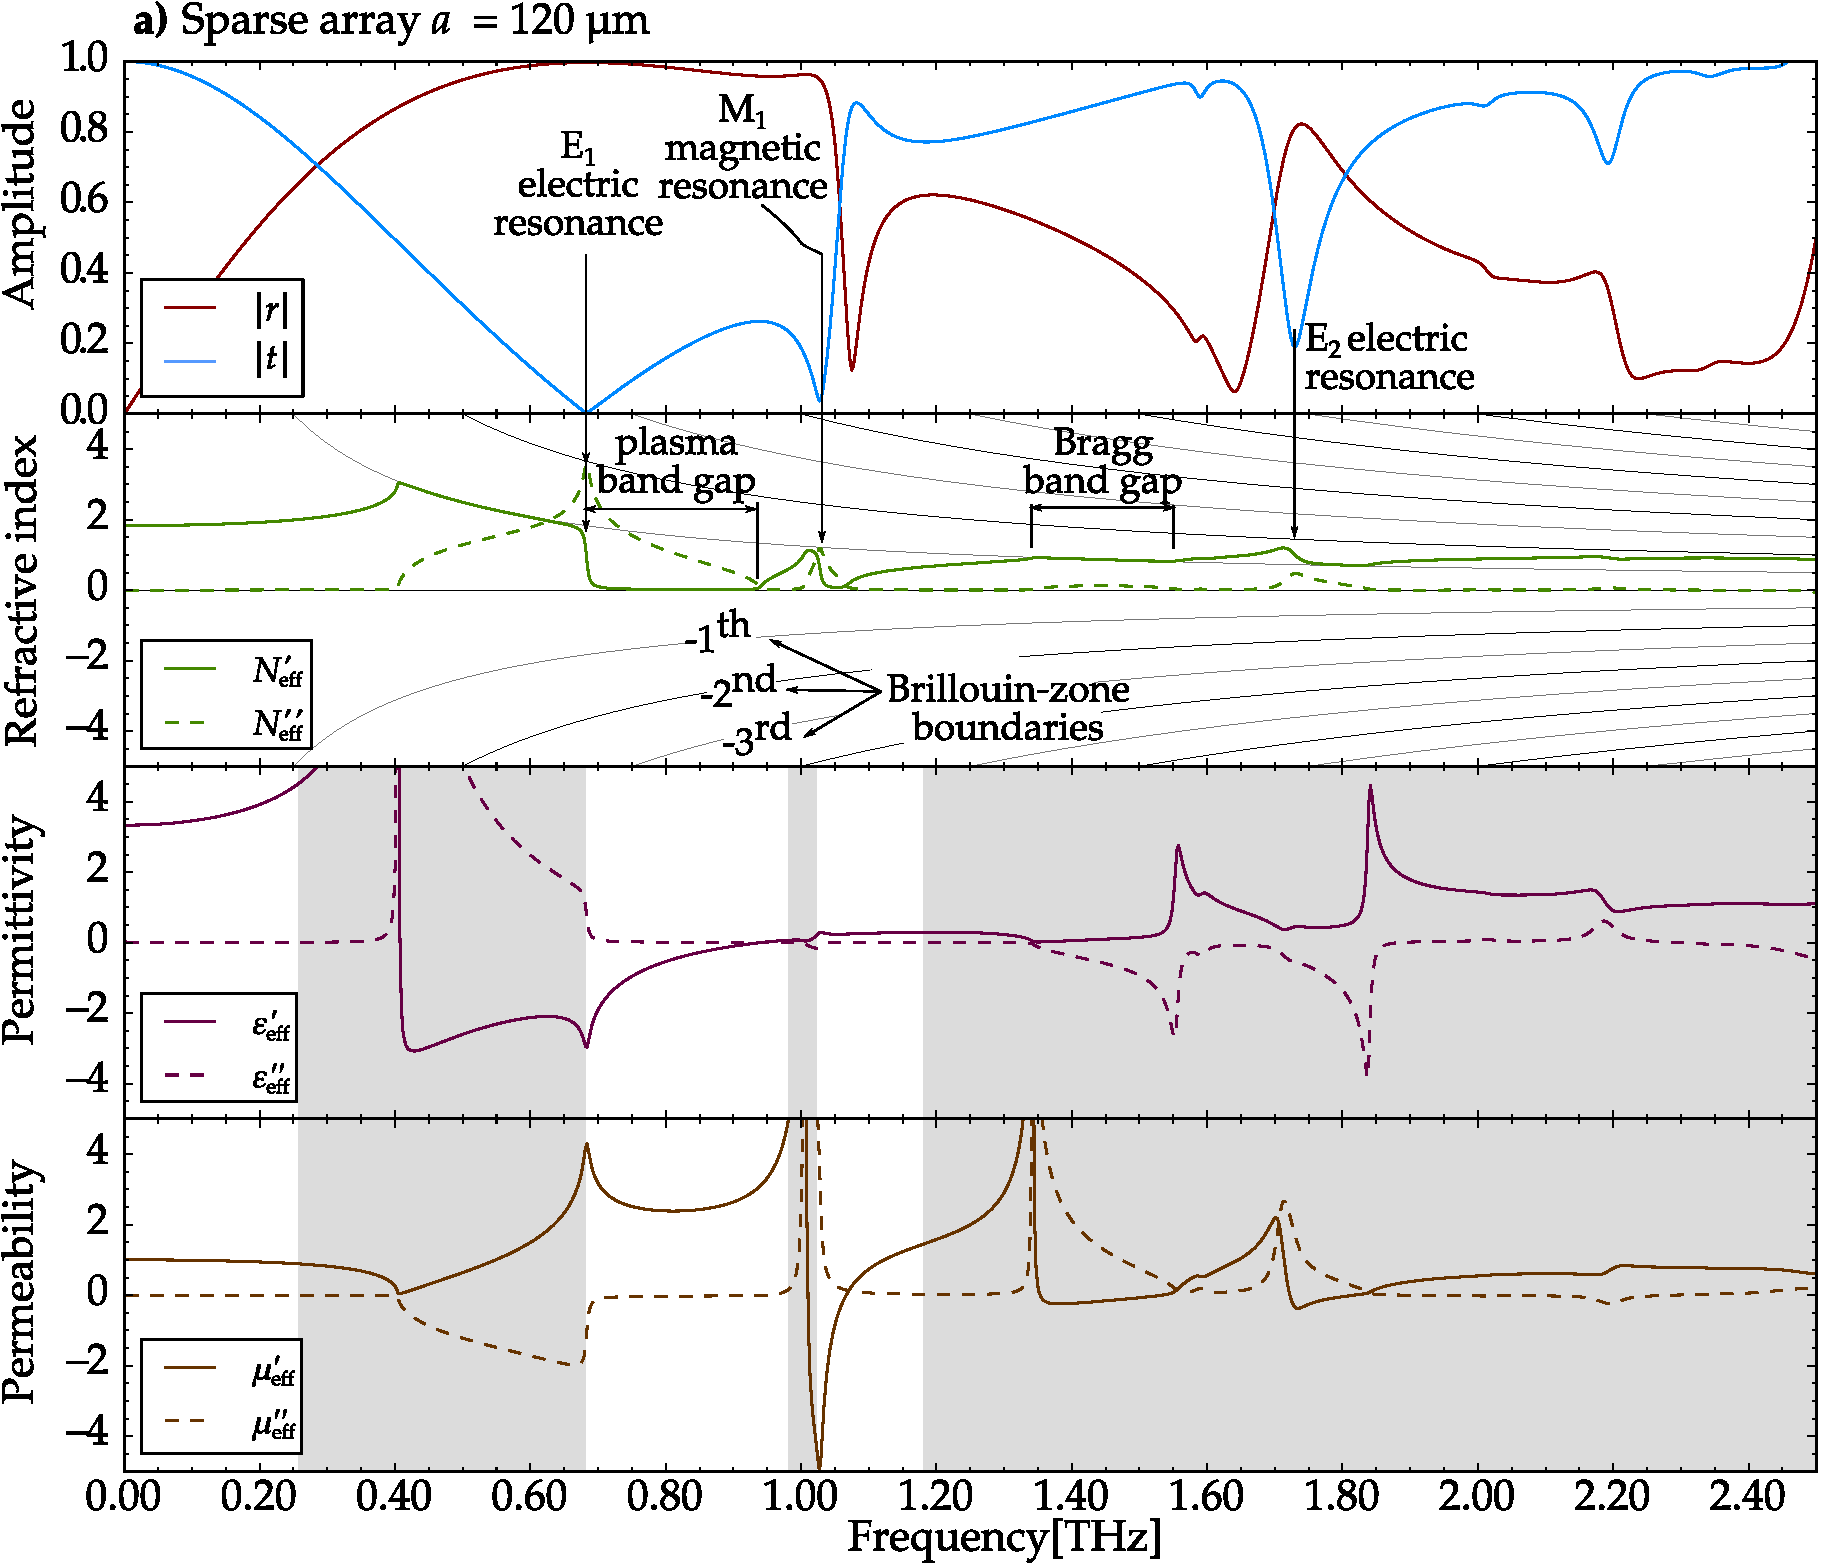
\includegraphics[width=10cm]{img/ERods_eps100_single_a120_FDTD.pdf} \end{figure} \clearpage
\begin{figure} \caption{img/ERods\_eps100\_triple\_a150a100a080\_FDTD.pdf}  \centering 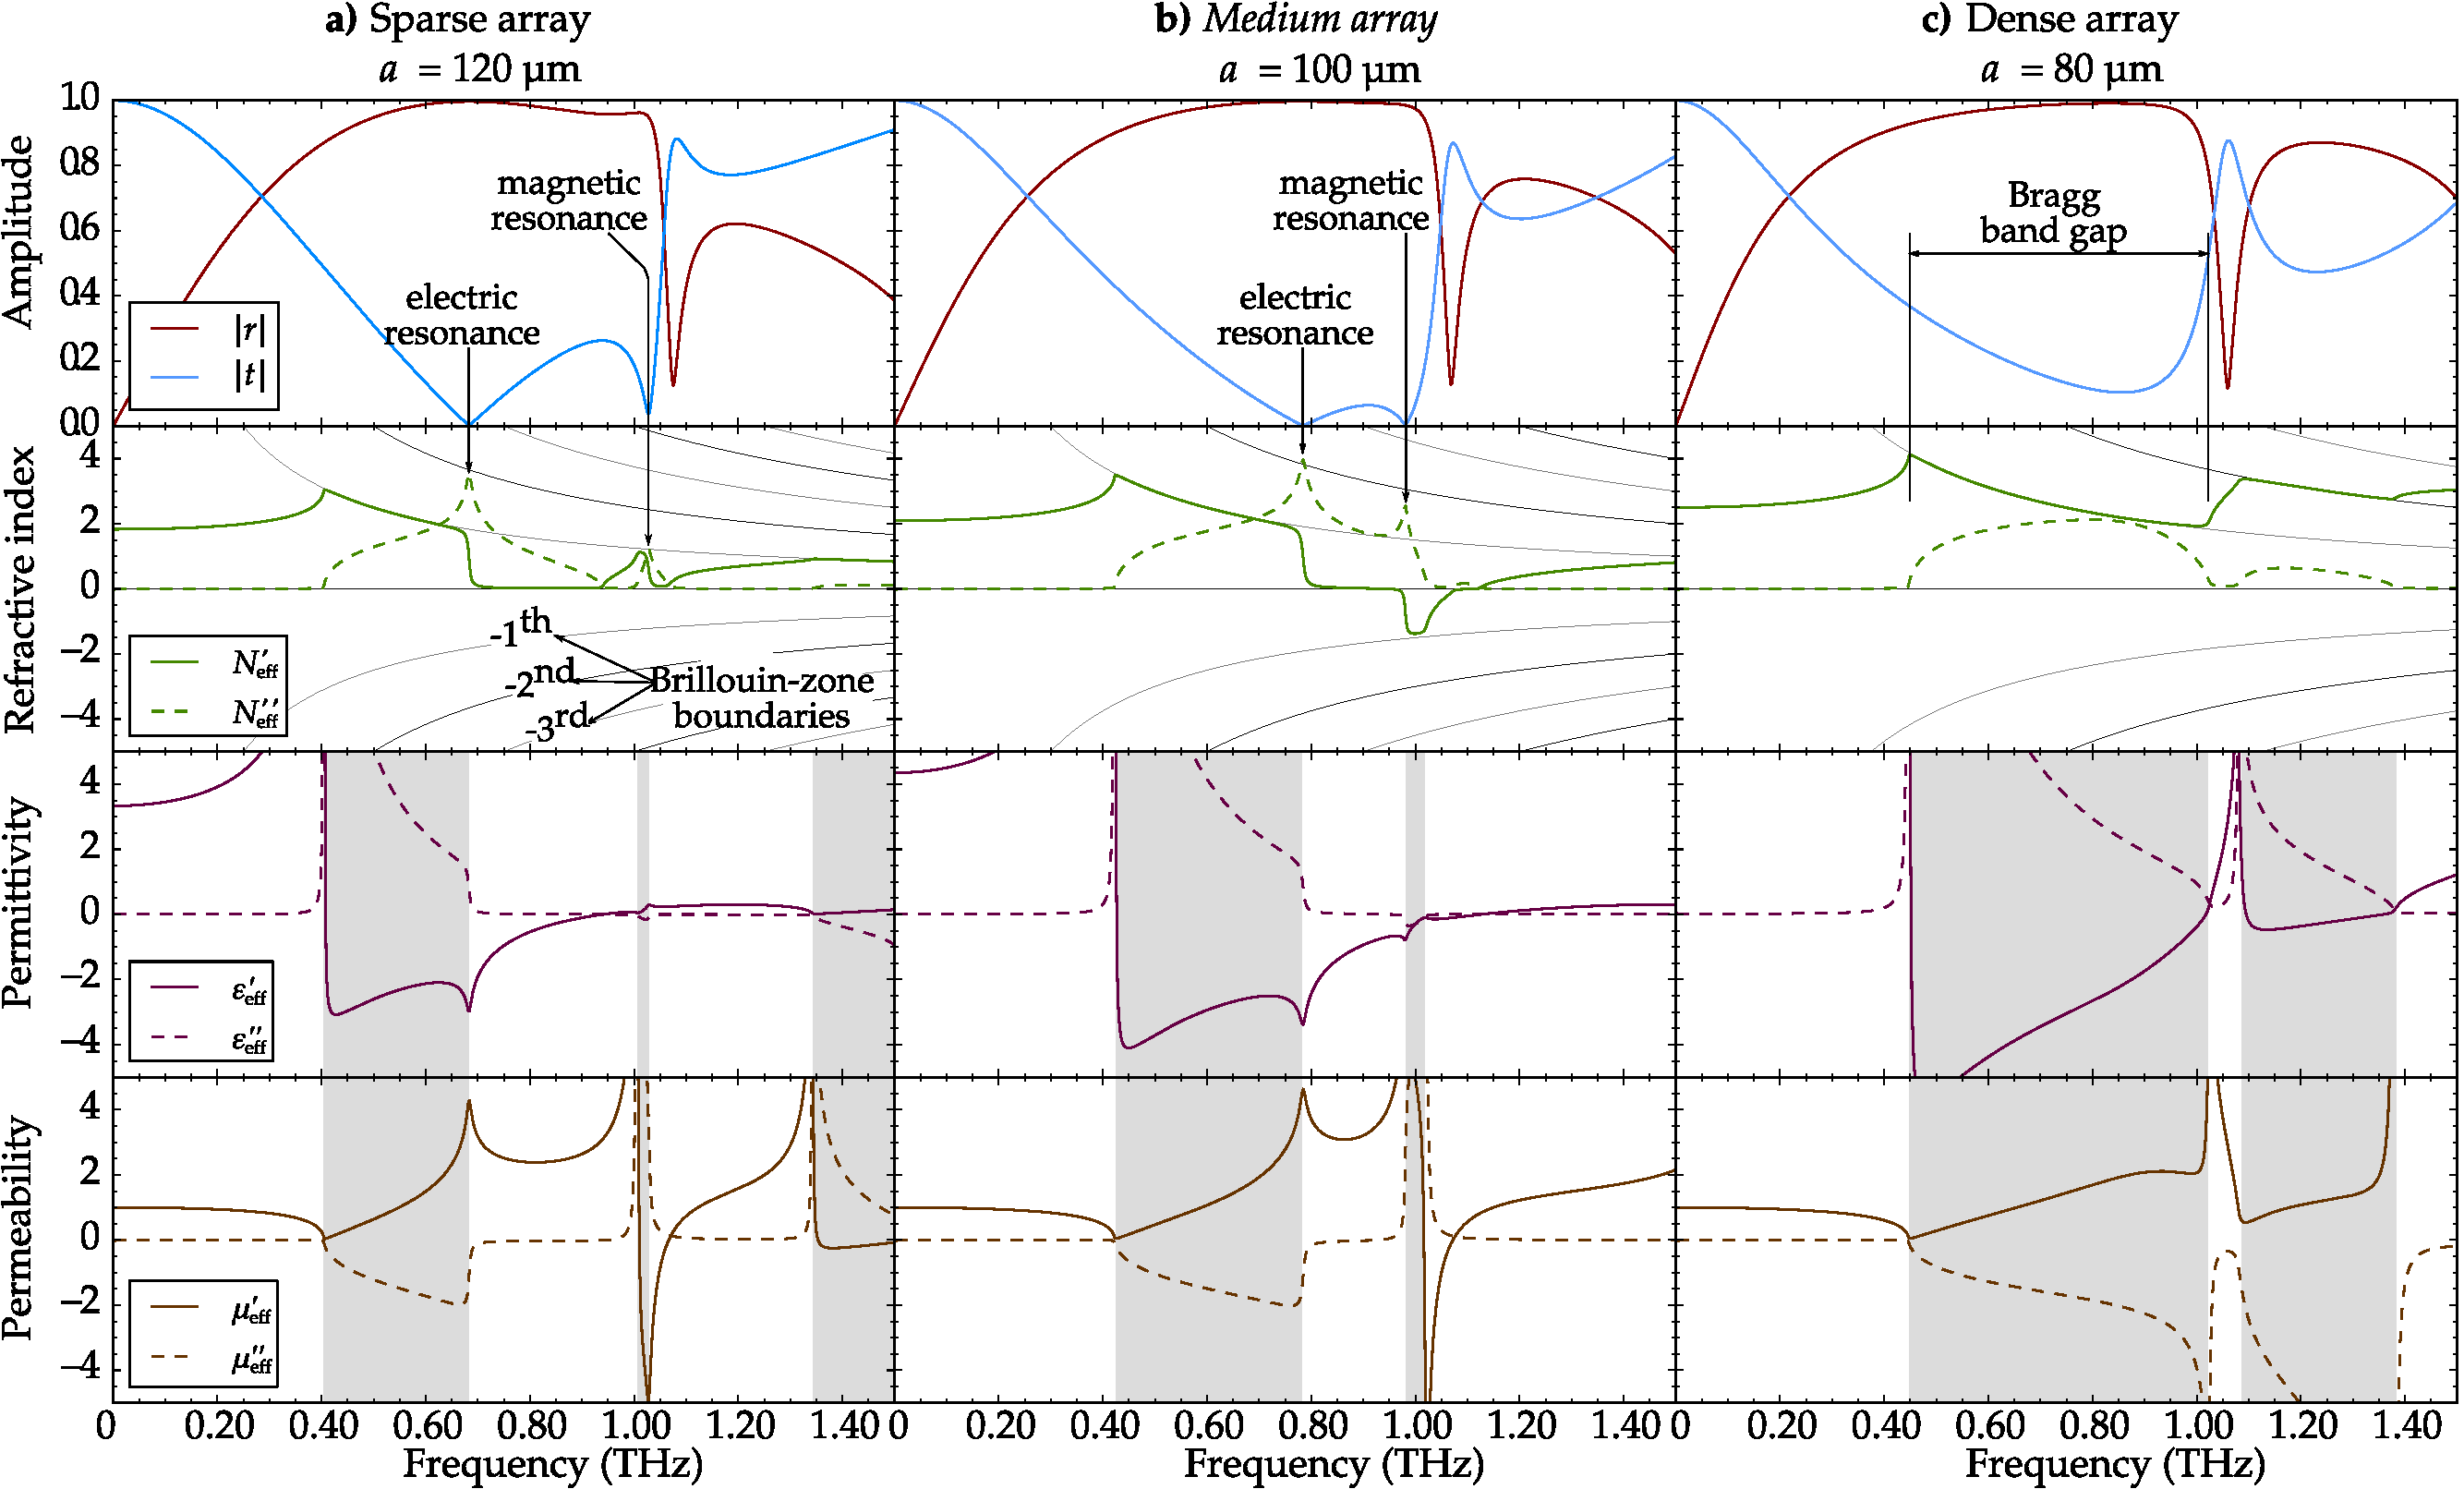
\includegraphics[width=10cm]{img/ERods_eps100_triple_a150a100a080_FDTD.pdf} \end{figure} \clearpage
\begin{figure} \caption{img/ERods\_forSeefeld\_sparserN\_denserN\_DrawnBands.pdf}  \centering 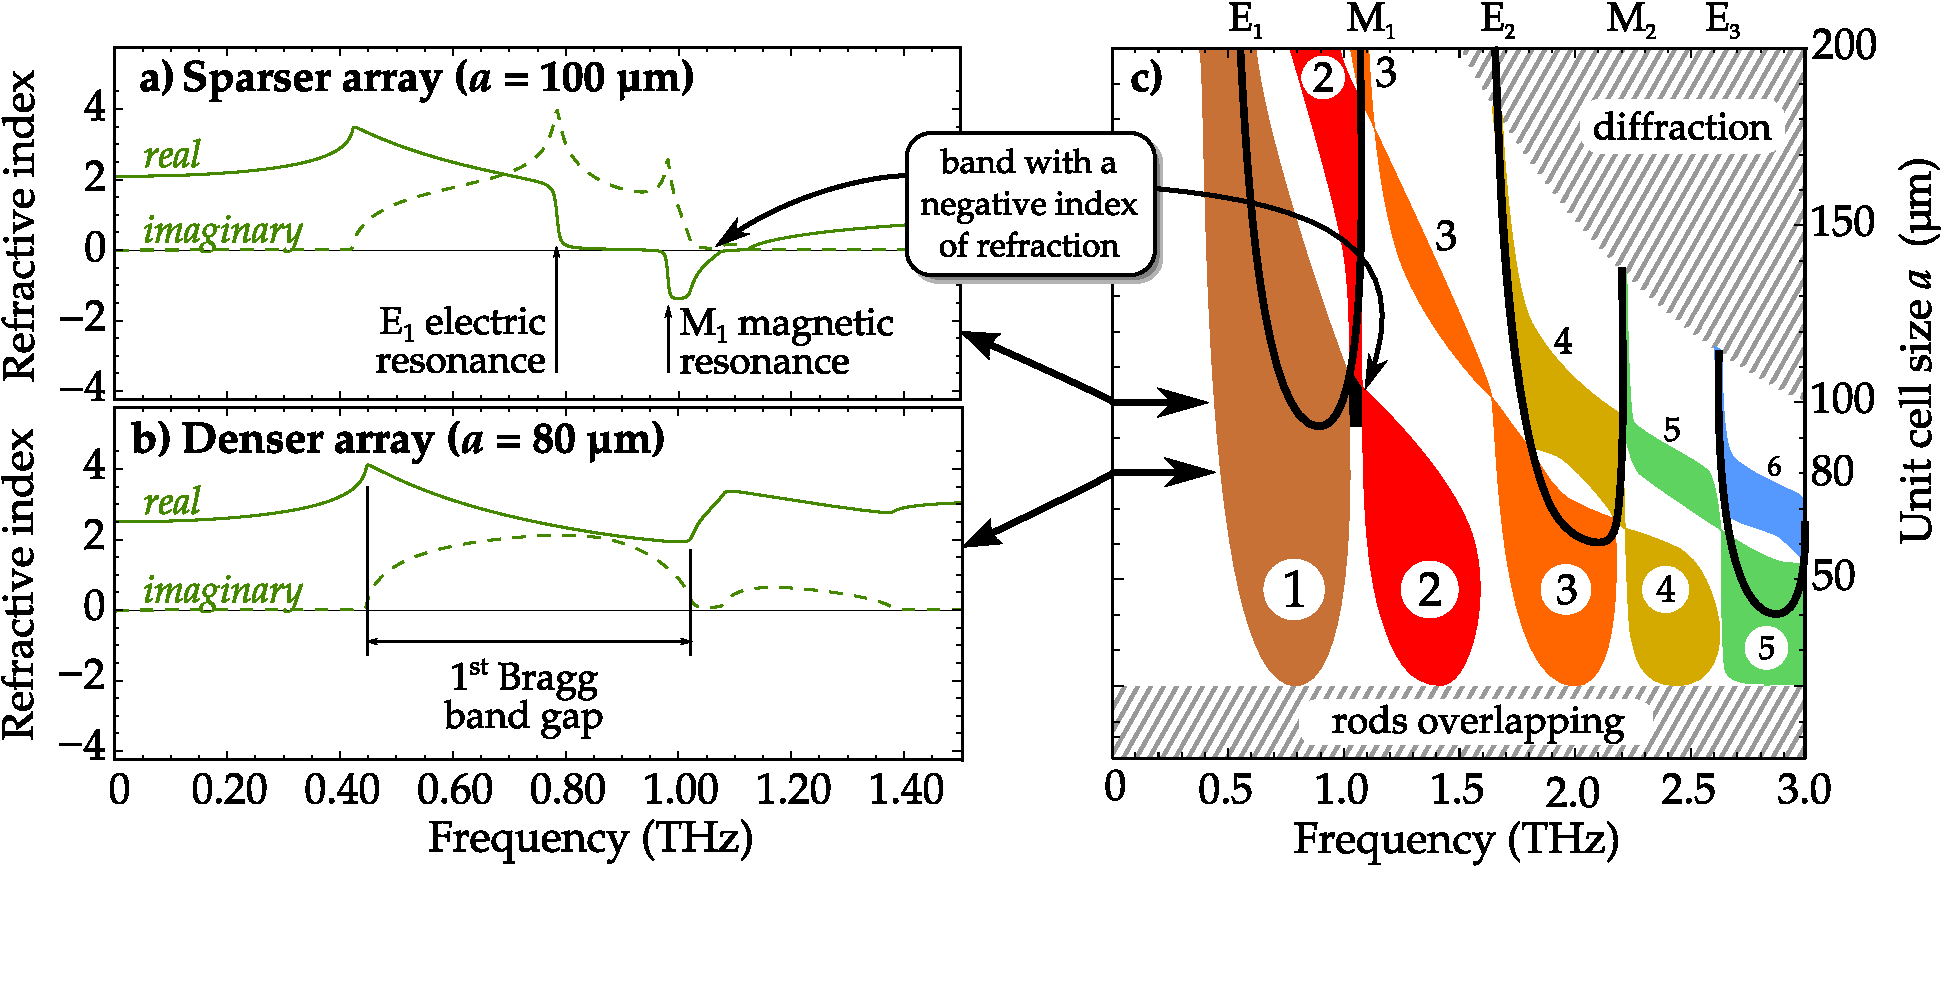
\includegraphics[width=10cm]{img/ERods_forSeefeld_sparserN_denserN_DrawnBands.pdf} \end{figure} \clearpage


\begin{figure} \caption{img/ERods\_sketch\_recordedline.pdf}  \centering  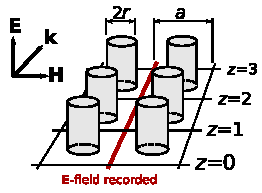
\includegraphics[width=10cm]{img/ERods_sketch_recordedline.pdf} \end{figure} \clearpage
\begin{figure} \caption{img/ERods\_eps100\_R10u5\_FXplot.pdf}  \centering 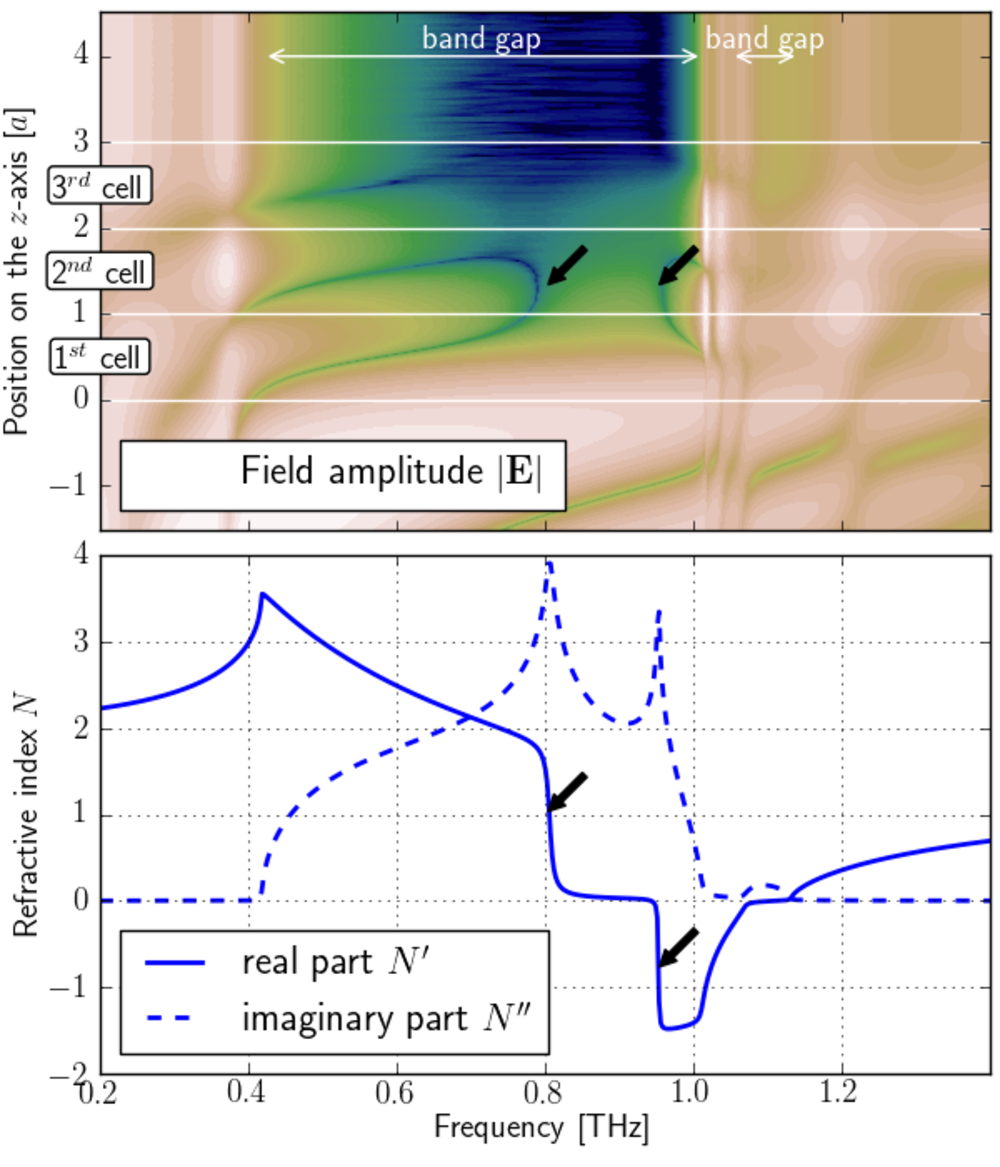
\includegraphics[width=10cm]{img/ERods_eps100_R10u5_FXplot.pdf} \end{figure} \clearpage
%}}}
\section{Metallic screen with a slit} % references to ->
\section{A fishnet - metallic screen with holes} % references to ->
%{{{
\begin{figure} \caption{img/fishnet.pdf}  \centering 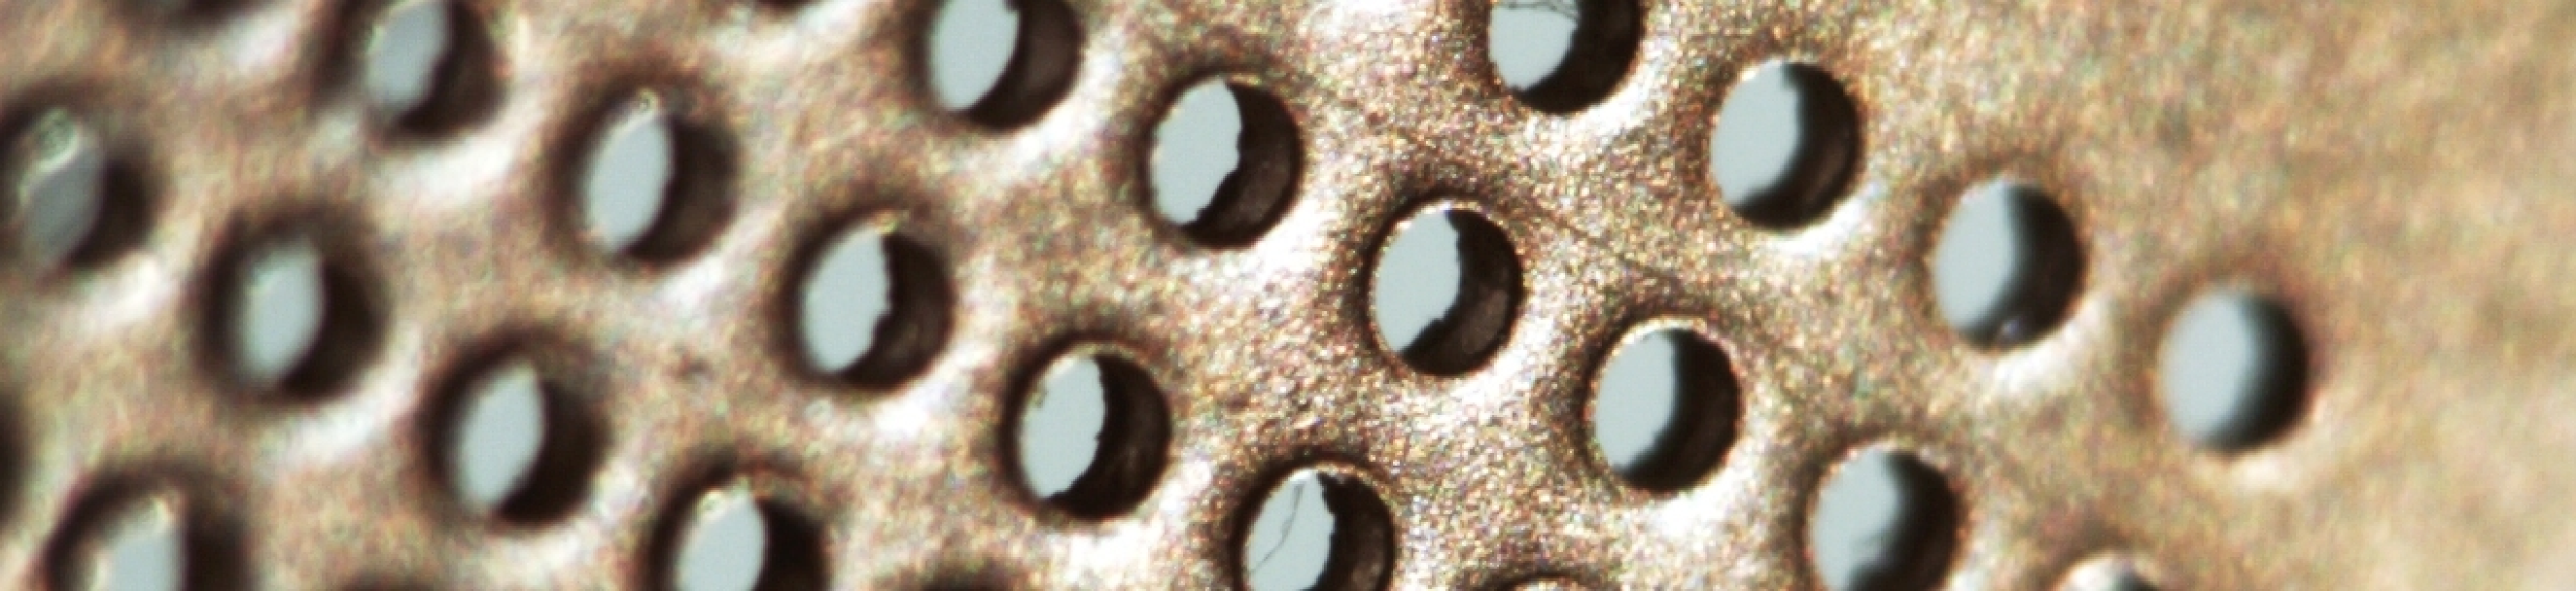
\includegraphics[width=10cm]{img/fishnet.pdf} \end{figure} \clearpage
%}}}

\section{Other structures} % plasmonic spheres (note: resonance width determined by gamma of the metal?)
\begin{figure} \caption{Modes in sphere-wire structure}  \centering 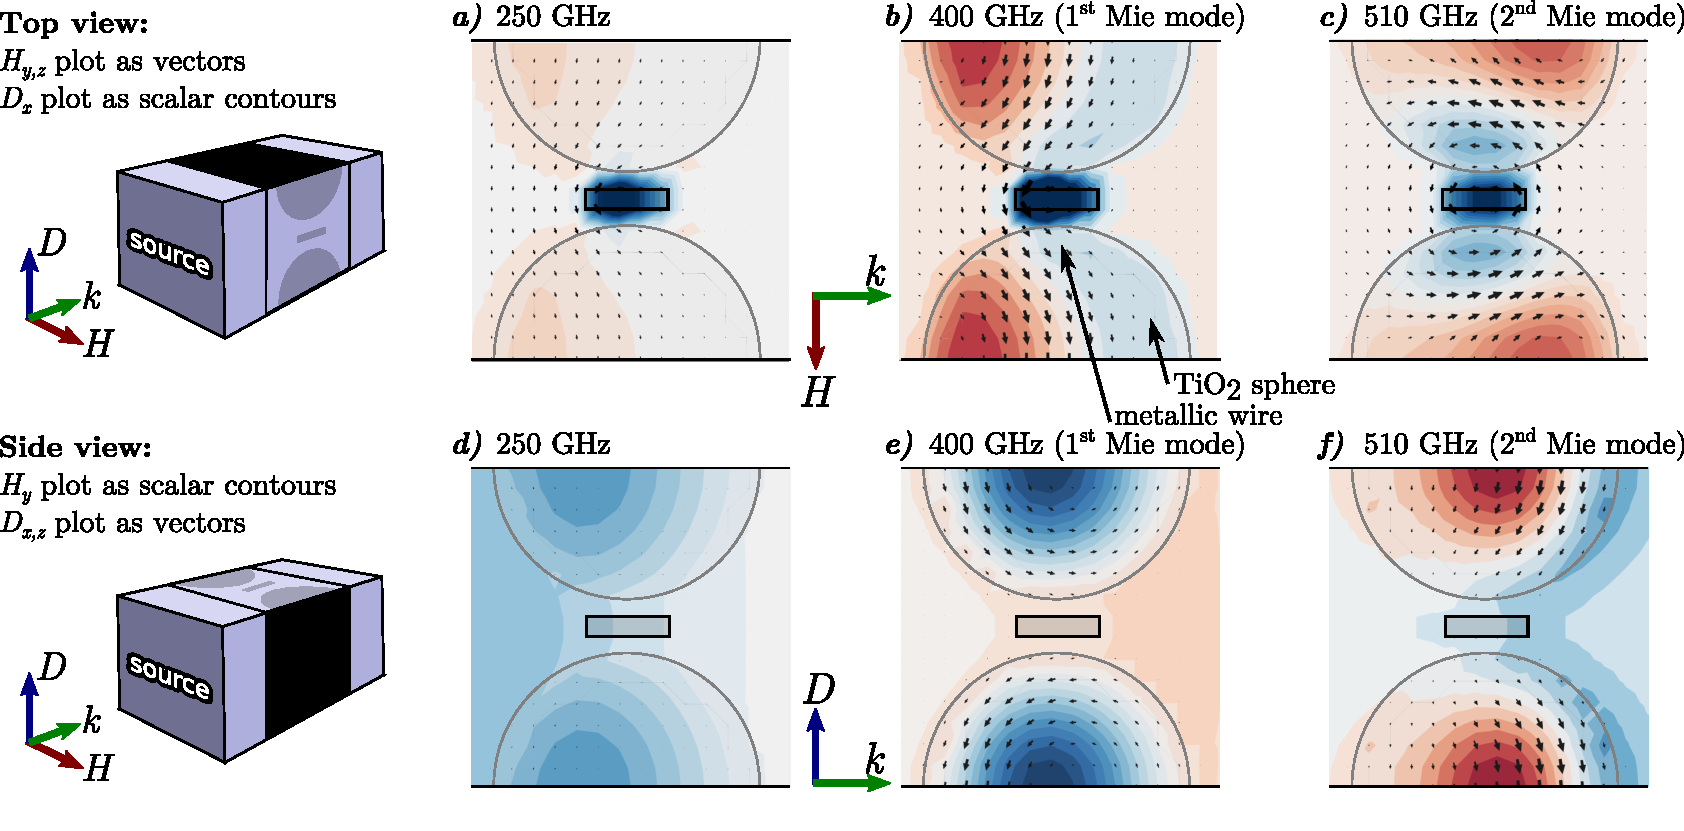
\includegraphics[width=10cm]{img/new/modes_Mag_and_El.pdf} \end{figure} \clearpage
\subsection{} % references to ->
\subsection{} % references to ->
\subsection{} % references to ->
\subsection{} % references to ->
\subsection{} % references to ->
